\documentclass[a4paper, 12pt]{article}

\title{
{	\vspace{3mm}
	\large Topological Data Analysis -- group project} \\
	\vspace{5mm}
	\hrule
	\vspace{3mm}
Sensors
	\vspace{3mm}
	\hrule
	\vspace{5mm}
}

\author{
	Nejc Ki\v sek,
	\v Zan Klane\v cek
}

\usepackage[utf8x]{inputenc}
\usepackage{float}
\usepackage{graphicx}
\usepackage{subcaption}
\usepackage{geometry}
\usepackage{amsfonts}
\usepackage{amsmath}
\usepackage{amssymb}
\usepackage{hyperref}
\newcommand{\vect}[1]{\boldsymbol{#1}}

\geometry{
	a4paper,
	left=30mm,
	top=35mm,
	right=30mm,
	bottom=35mm
}

\begin{document}
\maketitle

\vspace{8mm}


\section{Introduction}
In this project we are trying to find optimal parameters for a sensor network which covers the whole surface of the earth. The network is determined by two parameters: 
\begin{itemize}
	\item $r$, which is the distance over which the sensors can communicate with each other -- each sensor can communicate with another, if they are at most $r$ away.
	\item $R$, which is the radius of the surrounding area in shape of a circle, where the sensor can gather data.
\end{itemize}

\noindent Given the coordinates of each sensor, we have to determine the lowest possible parameters $r$ and $R$ so that:

\begin{itemize}
	\item {the sensor network is connected,}
	\item {the sensor network covers the whole sphere (surface of the Earth).}
\end{itemize}
Furthermore, once the parameters $r$ and $R$ are established, we have to find obsolete sensors -- the sensors whose removal would not change the connectivity and coverage of the network. 

Lastly, a data generator that distributes $n$ points evenly on the surface of a sphere will be described. Parameters $r$ and $R$ of the sensor network on the points generated by this generatos will be as small as possible.
\section{Topological solution}

In this section theoretical background for our problem is described. Firstly, if we want to achieve sensor network connectivity (all sensors are connected), we should have a look at Vietoris-Rips complex. The properties of Vietoris-Rips are described with following relations:

\begin{itemize}
	\item {sensors: S $\big(S_i = (r_i, \phi_i, \theta_i)\big)$,}
	\item {sensor connections $\{S_i, S_j\} \subset S; d(S_i, S_j) \leq r$,}
	\item {$F \subset S$ is a simplex in $VR_r(S)$, if diam $F \leq r$,}
\end{itemize} 
where $r$ is the parameter of the Vietoris-Rips complex and $d(S_i, S_j)$ is Euclidean distance between two sensors. We can see that two vertices in thr Vietoris-Rips complex will be connected if they are at most $r$ away, which is is also the requirement for them to be communicate. 

To get a connected sensor network, such $r$ (as small as possible) should be determined, that Vietoris-Rips graph on a given distribution of sensors is connected (i.e. has one component).
\\

Secondly, if we want to achieve coverage of the entire sphere, Čech complex will come in handy:

\begin{itemize}
	\item {sensors: S $\big(S_i = (r_i, \phi_i, \theta_i)\big)$,}
	\item {$B_R(x)$ closed ball with radius $R$ around $x$,}
	\item {$C_R = \{\sigma \subset S,\cap_{x\in \sigma}B_R(x) \neq \emptyset \}$.
	}
\end{itemize}

 Three vertices in a Čech complex form a triangle if the balls with radius $R$ around them have a common intersection. From that follows that every triangle in the Čech complex represents an area that is completely covered by the sensors. This means that the \v Cech complex on our ideal sensor network covers the whole surface with triangles and is therefore homeomorphic to a sphere. 

In practice, we ignored higher dimensional vertices, because they only appear when more than three sensors are very close together, which is not an issue. We therefore just looked at the first 2 Betti numbers: $\beta_0$, which is the number of components and should be 1 and $\beta_1$, which is the number of cycles or holes in the complex and should be 0.

\clearpage

\section{Connectivity}
To determine if the sensor network is connected, we computed Vietoris-Rips complexes with different $r$ parameters and observed the graphs represented by points and edges of such complexes. We wanted the resulting graph to have just 1 component.

\begin{figure}[H]
        \centering
        \makebox[\linewidth][c]{
        	\centering
            \begin{subfigure}[b]{0.50\textwidth}
                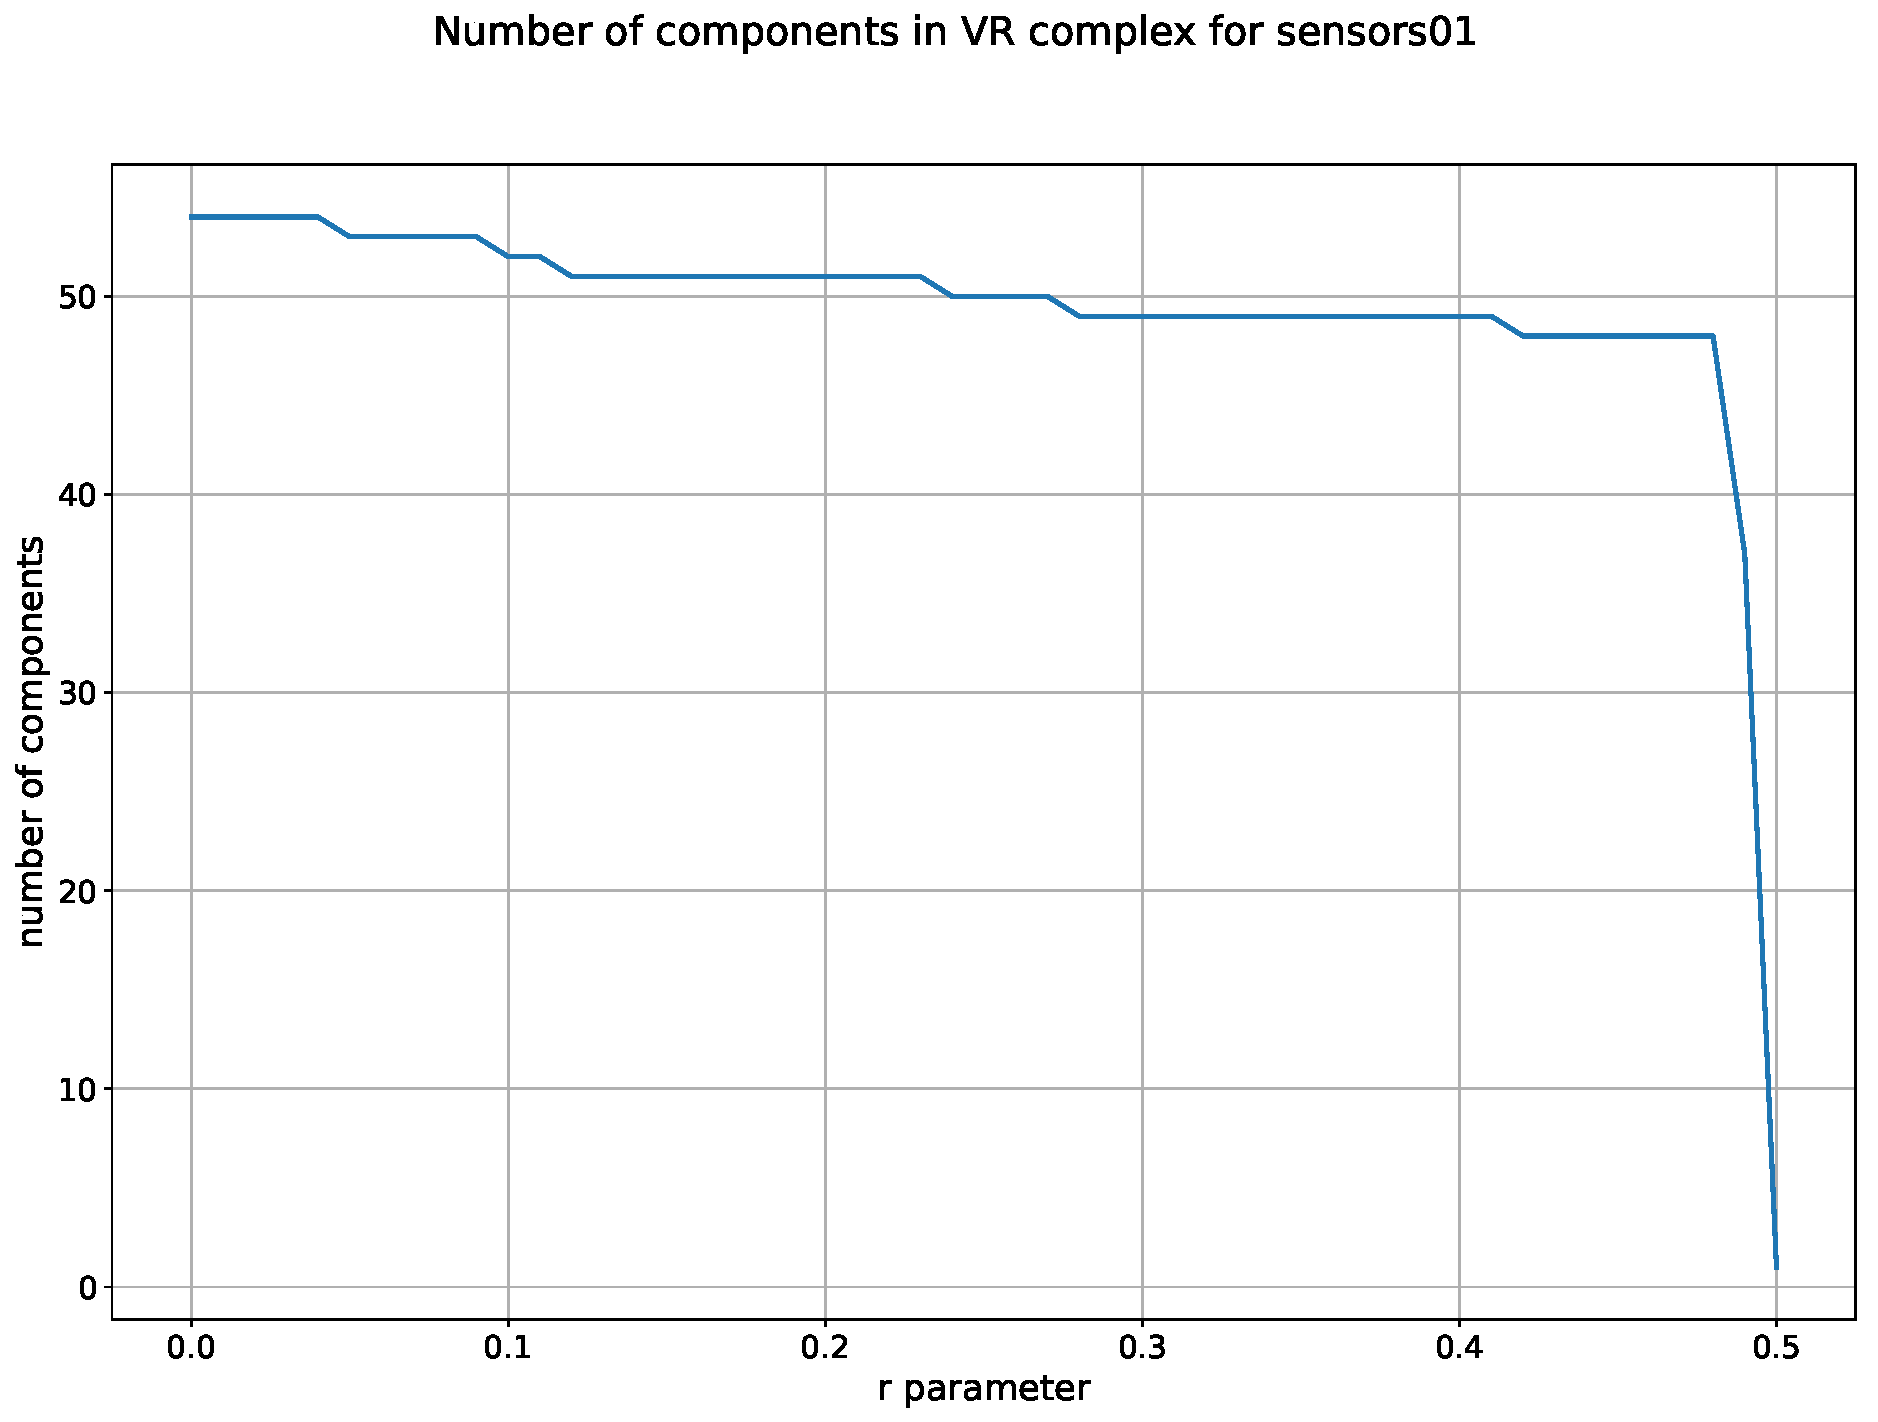
\includegraphics[width=\textwidth]{../images/plot_vr_sensors01}
            \end{subfigure}
            \begin{subfigure}[b]{0.50\textwidth}
                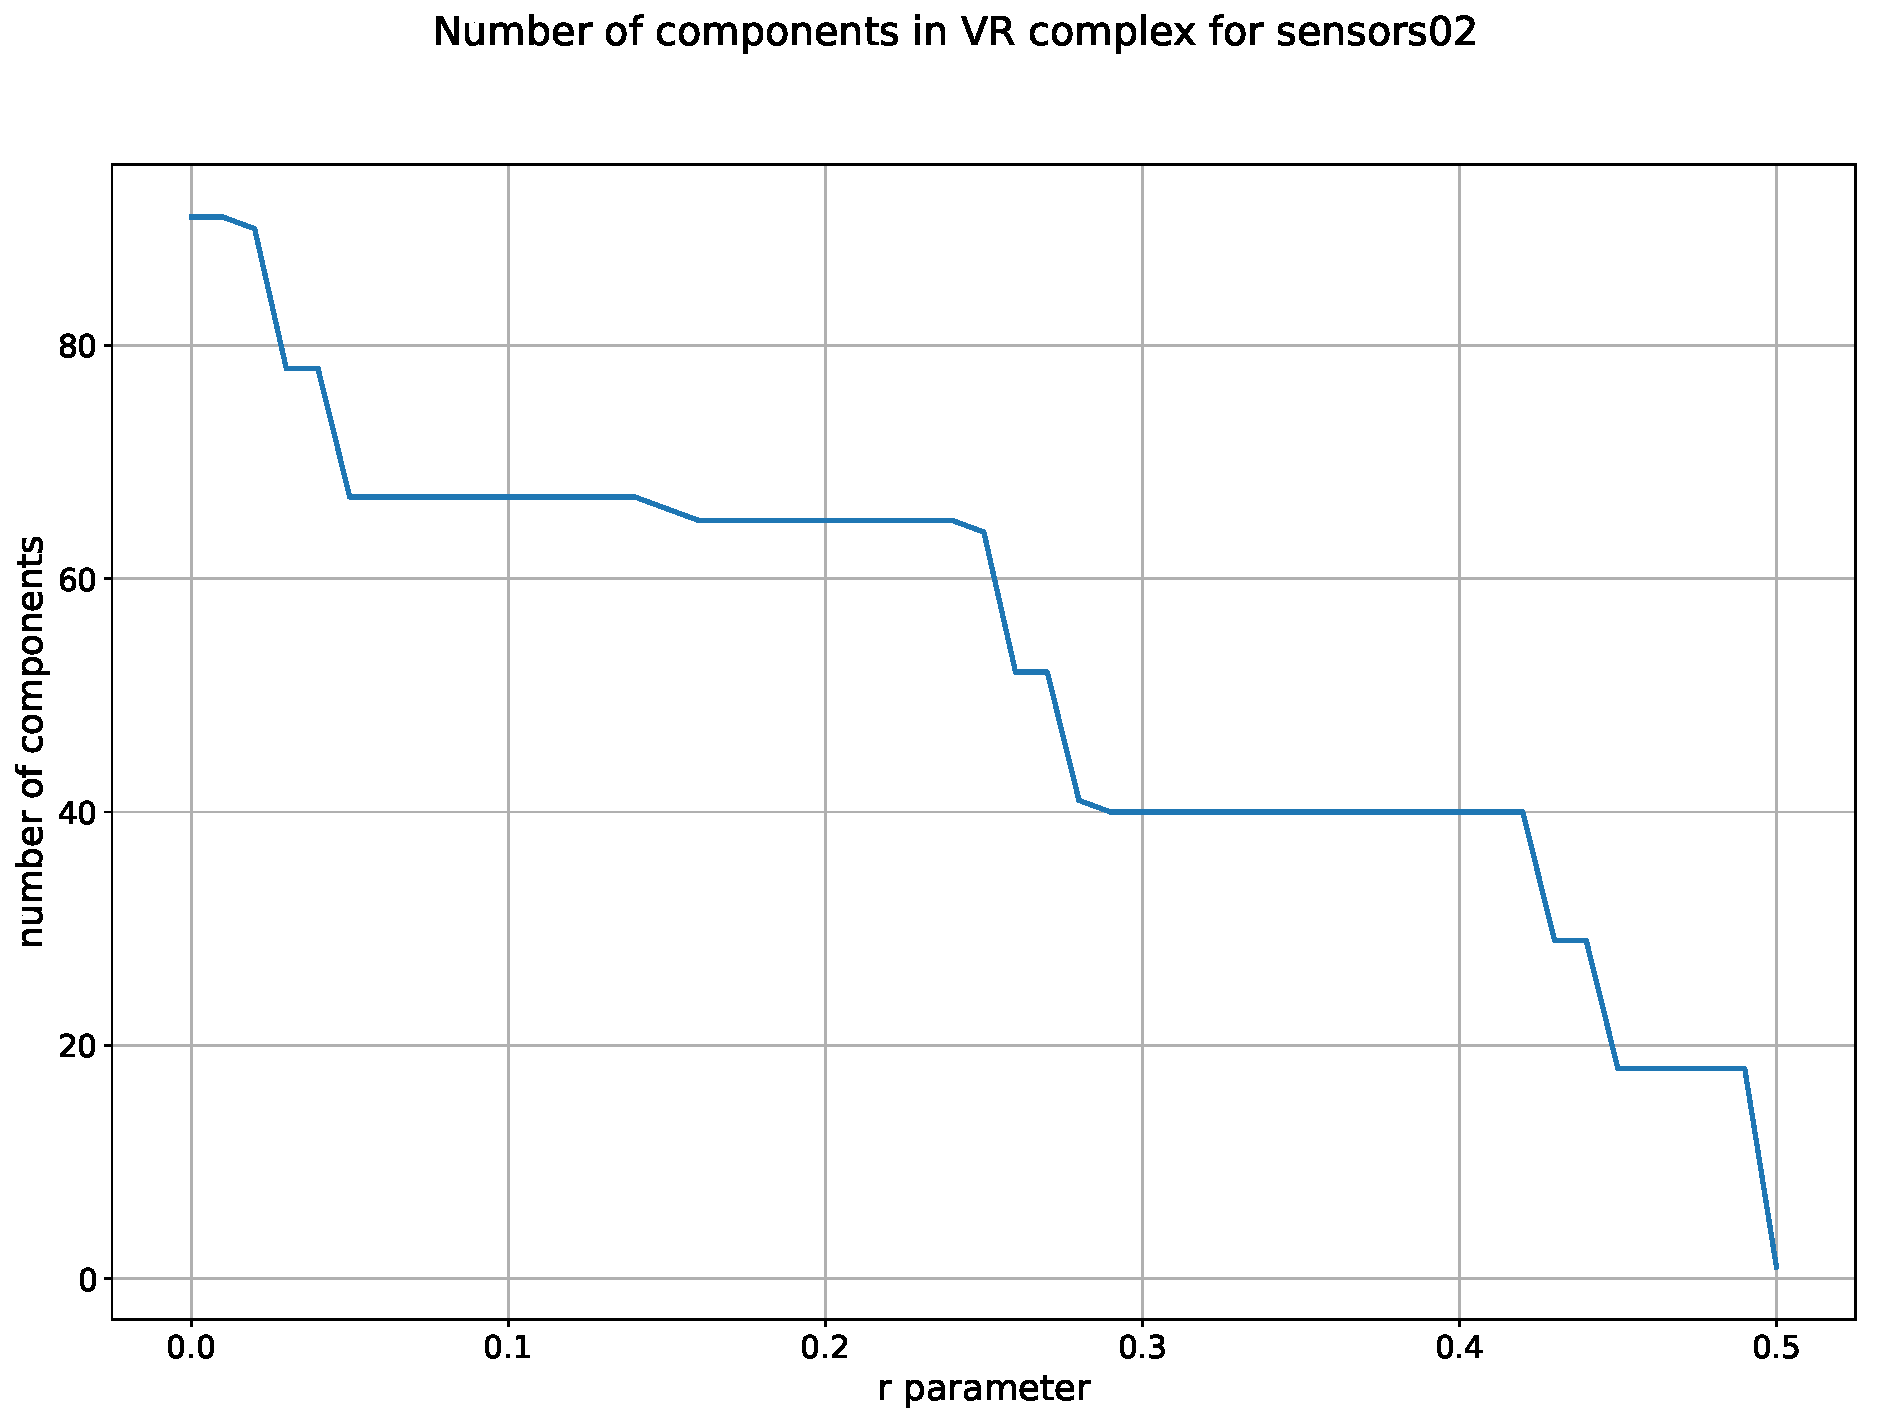
\includegraphics[width=\textwidth]{../images/plot_vr_sensors02}
            \end{subfigure}
        }
        \caption{Number of components as we increase the $r$ parameter}
        \label{plot-vr}
\end{figure}

In Figure \ref{plot-vr} we can see how the number of components changes as we increase the $r$. 
In the first dataset, the points were evenly distributed on the sphere, so most of them had roughly equal spacing between them -- we can see that the number of components decreases slowly at first, and quickly drops to 1 when we approach $0.5$. 
In the second dataset, points around the equator were further apart than those around the poles -- we can see that the number of components gradually decreases.

\begin{figure}[H]
        \centering
        \makebox[\linewidth][c]{
        	\centering
            \begin{subfigure}[b]{0.50\textwidth}
                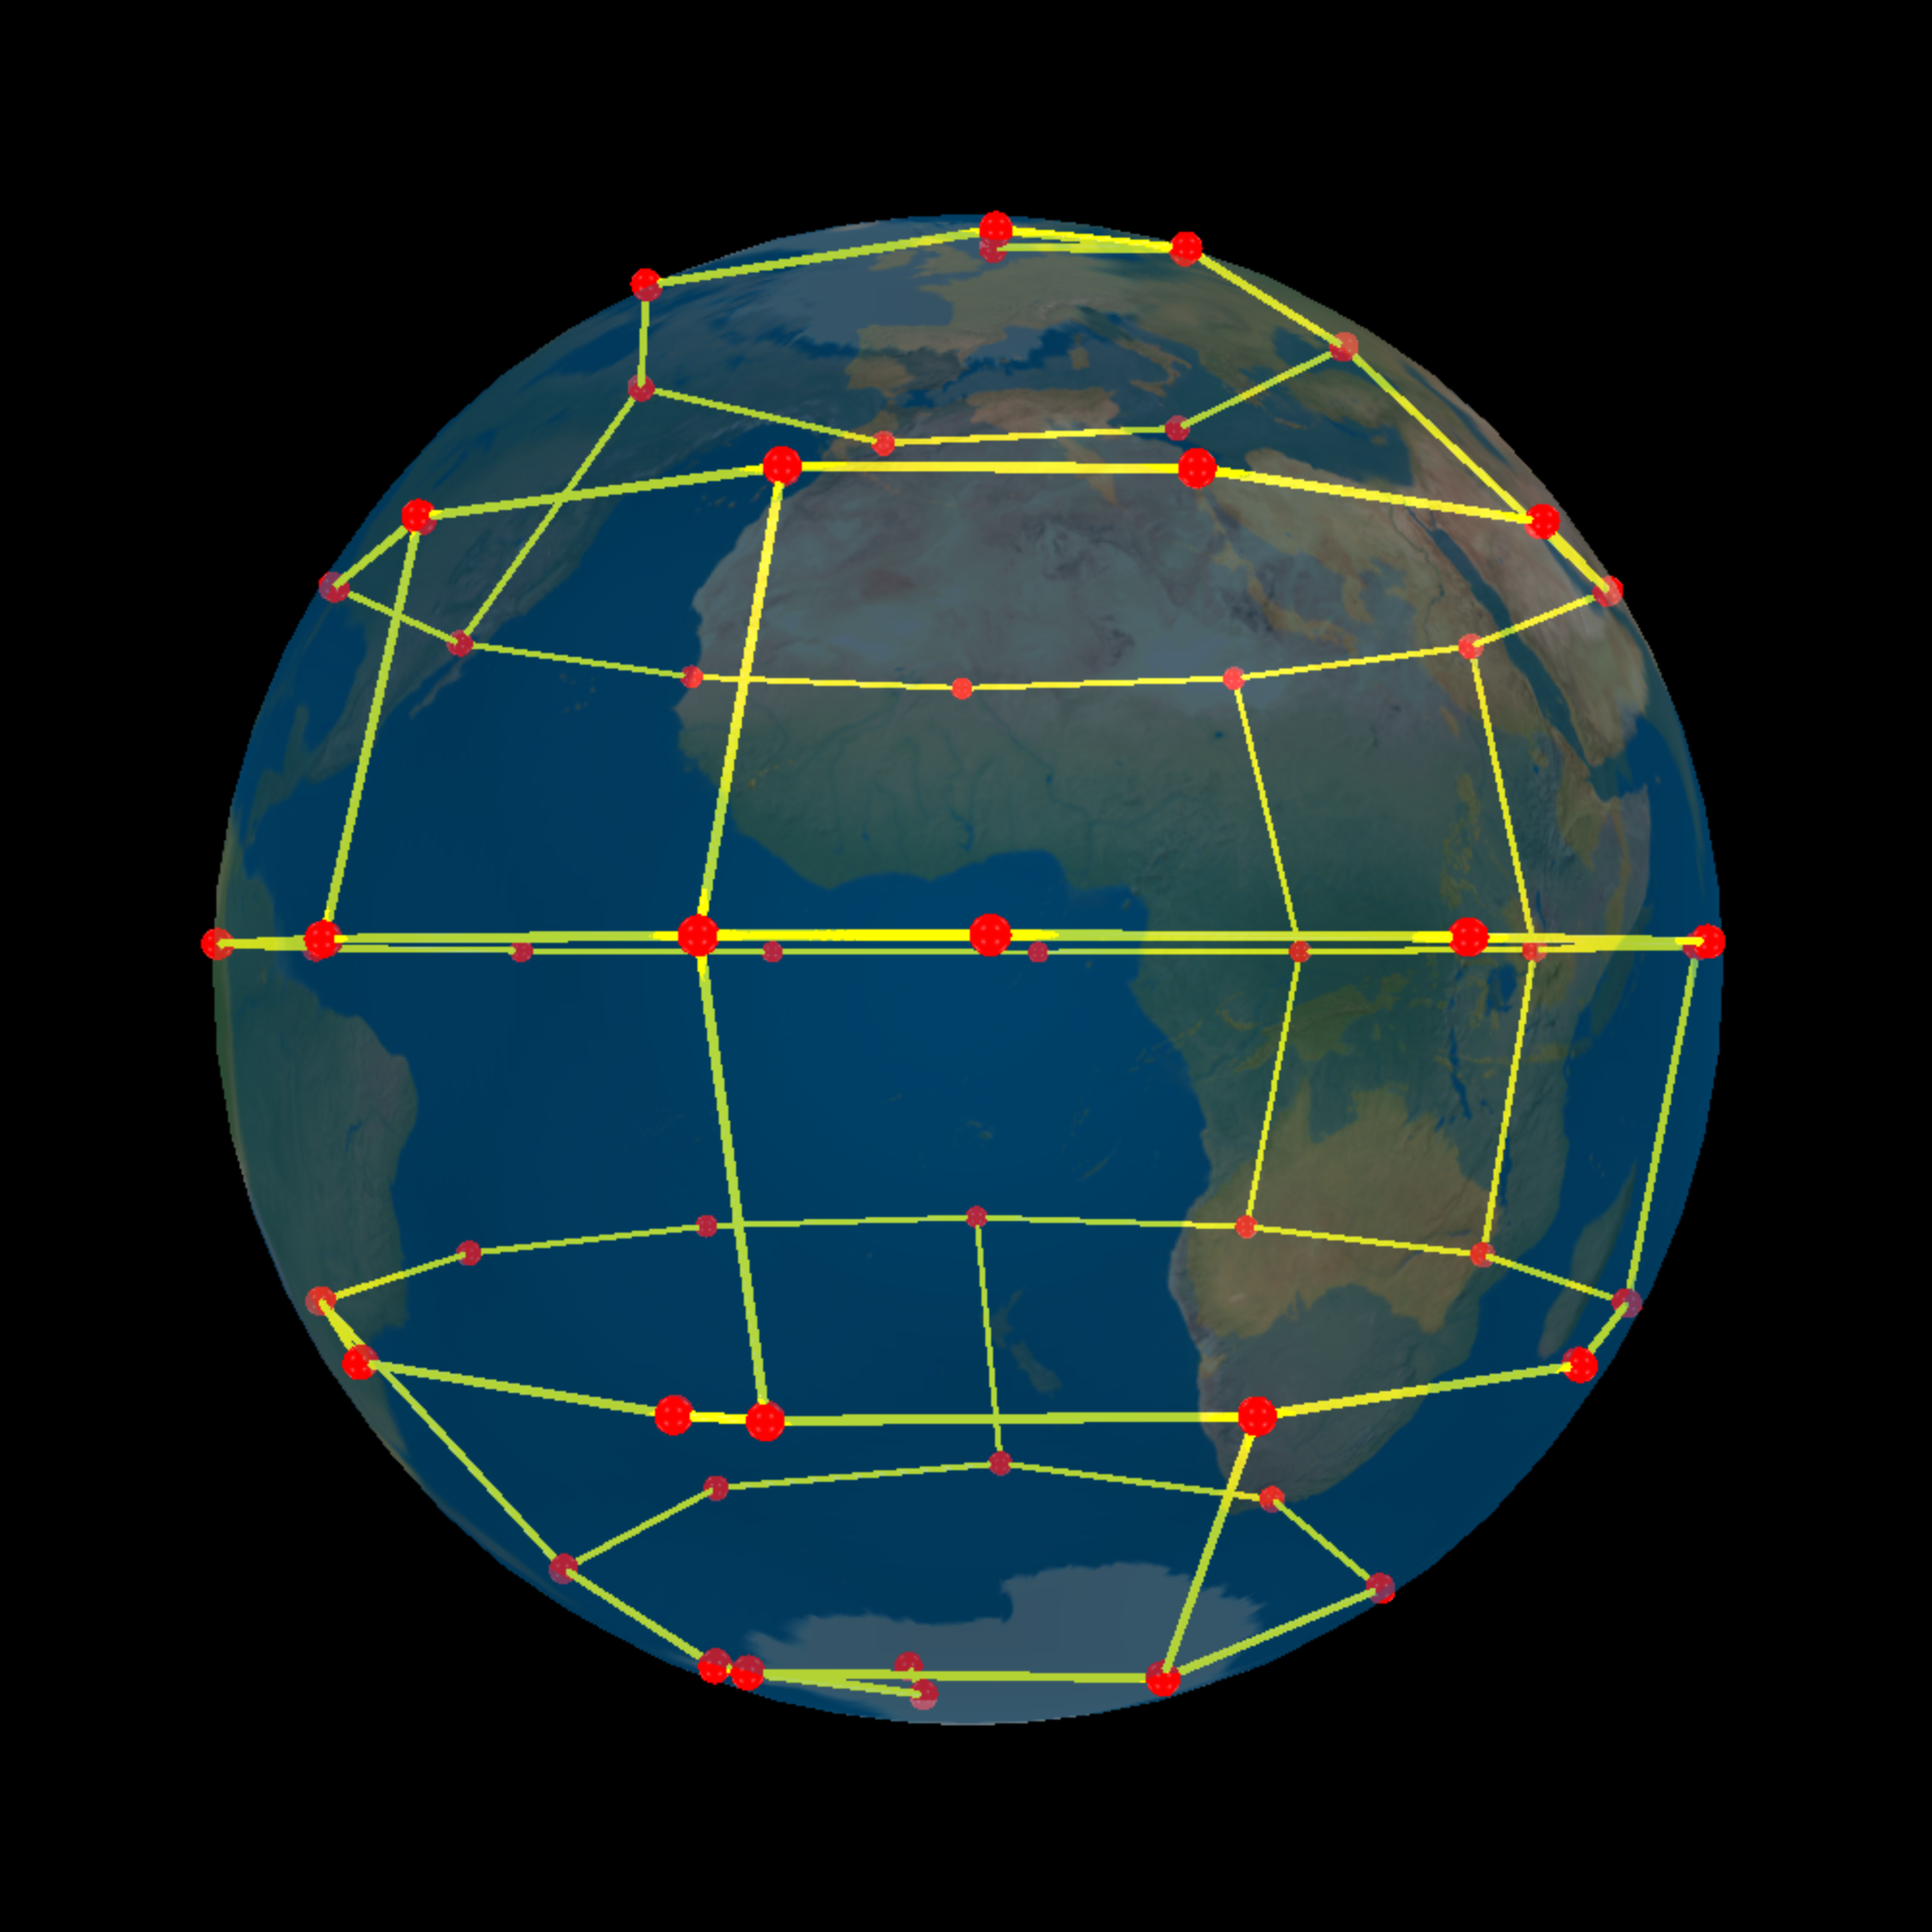
\includegraphics[width=\textwidth]{../images/connections01}
                \caption{sensors01.txt ($r=0.5$)}
            \end{subfigure}
            \begin{subfigure}[b]{0.50\textwidth}
                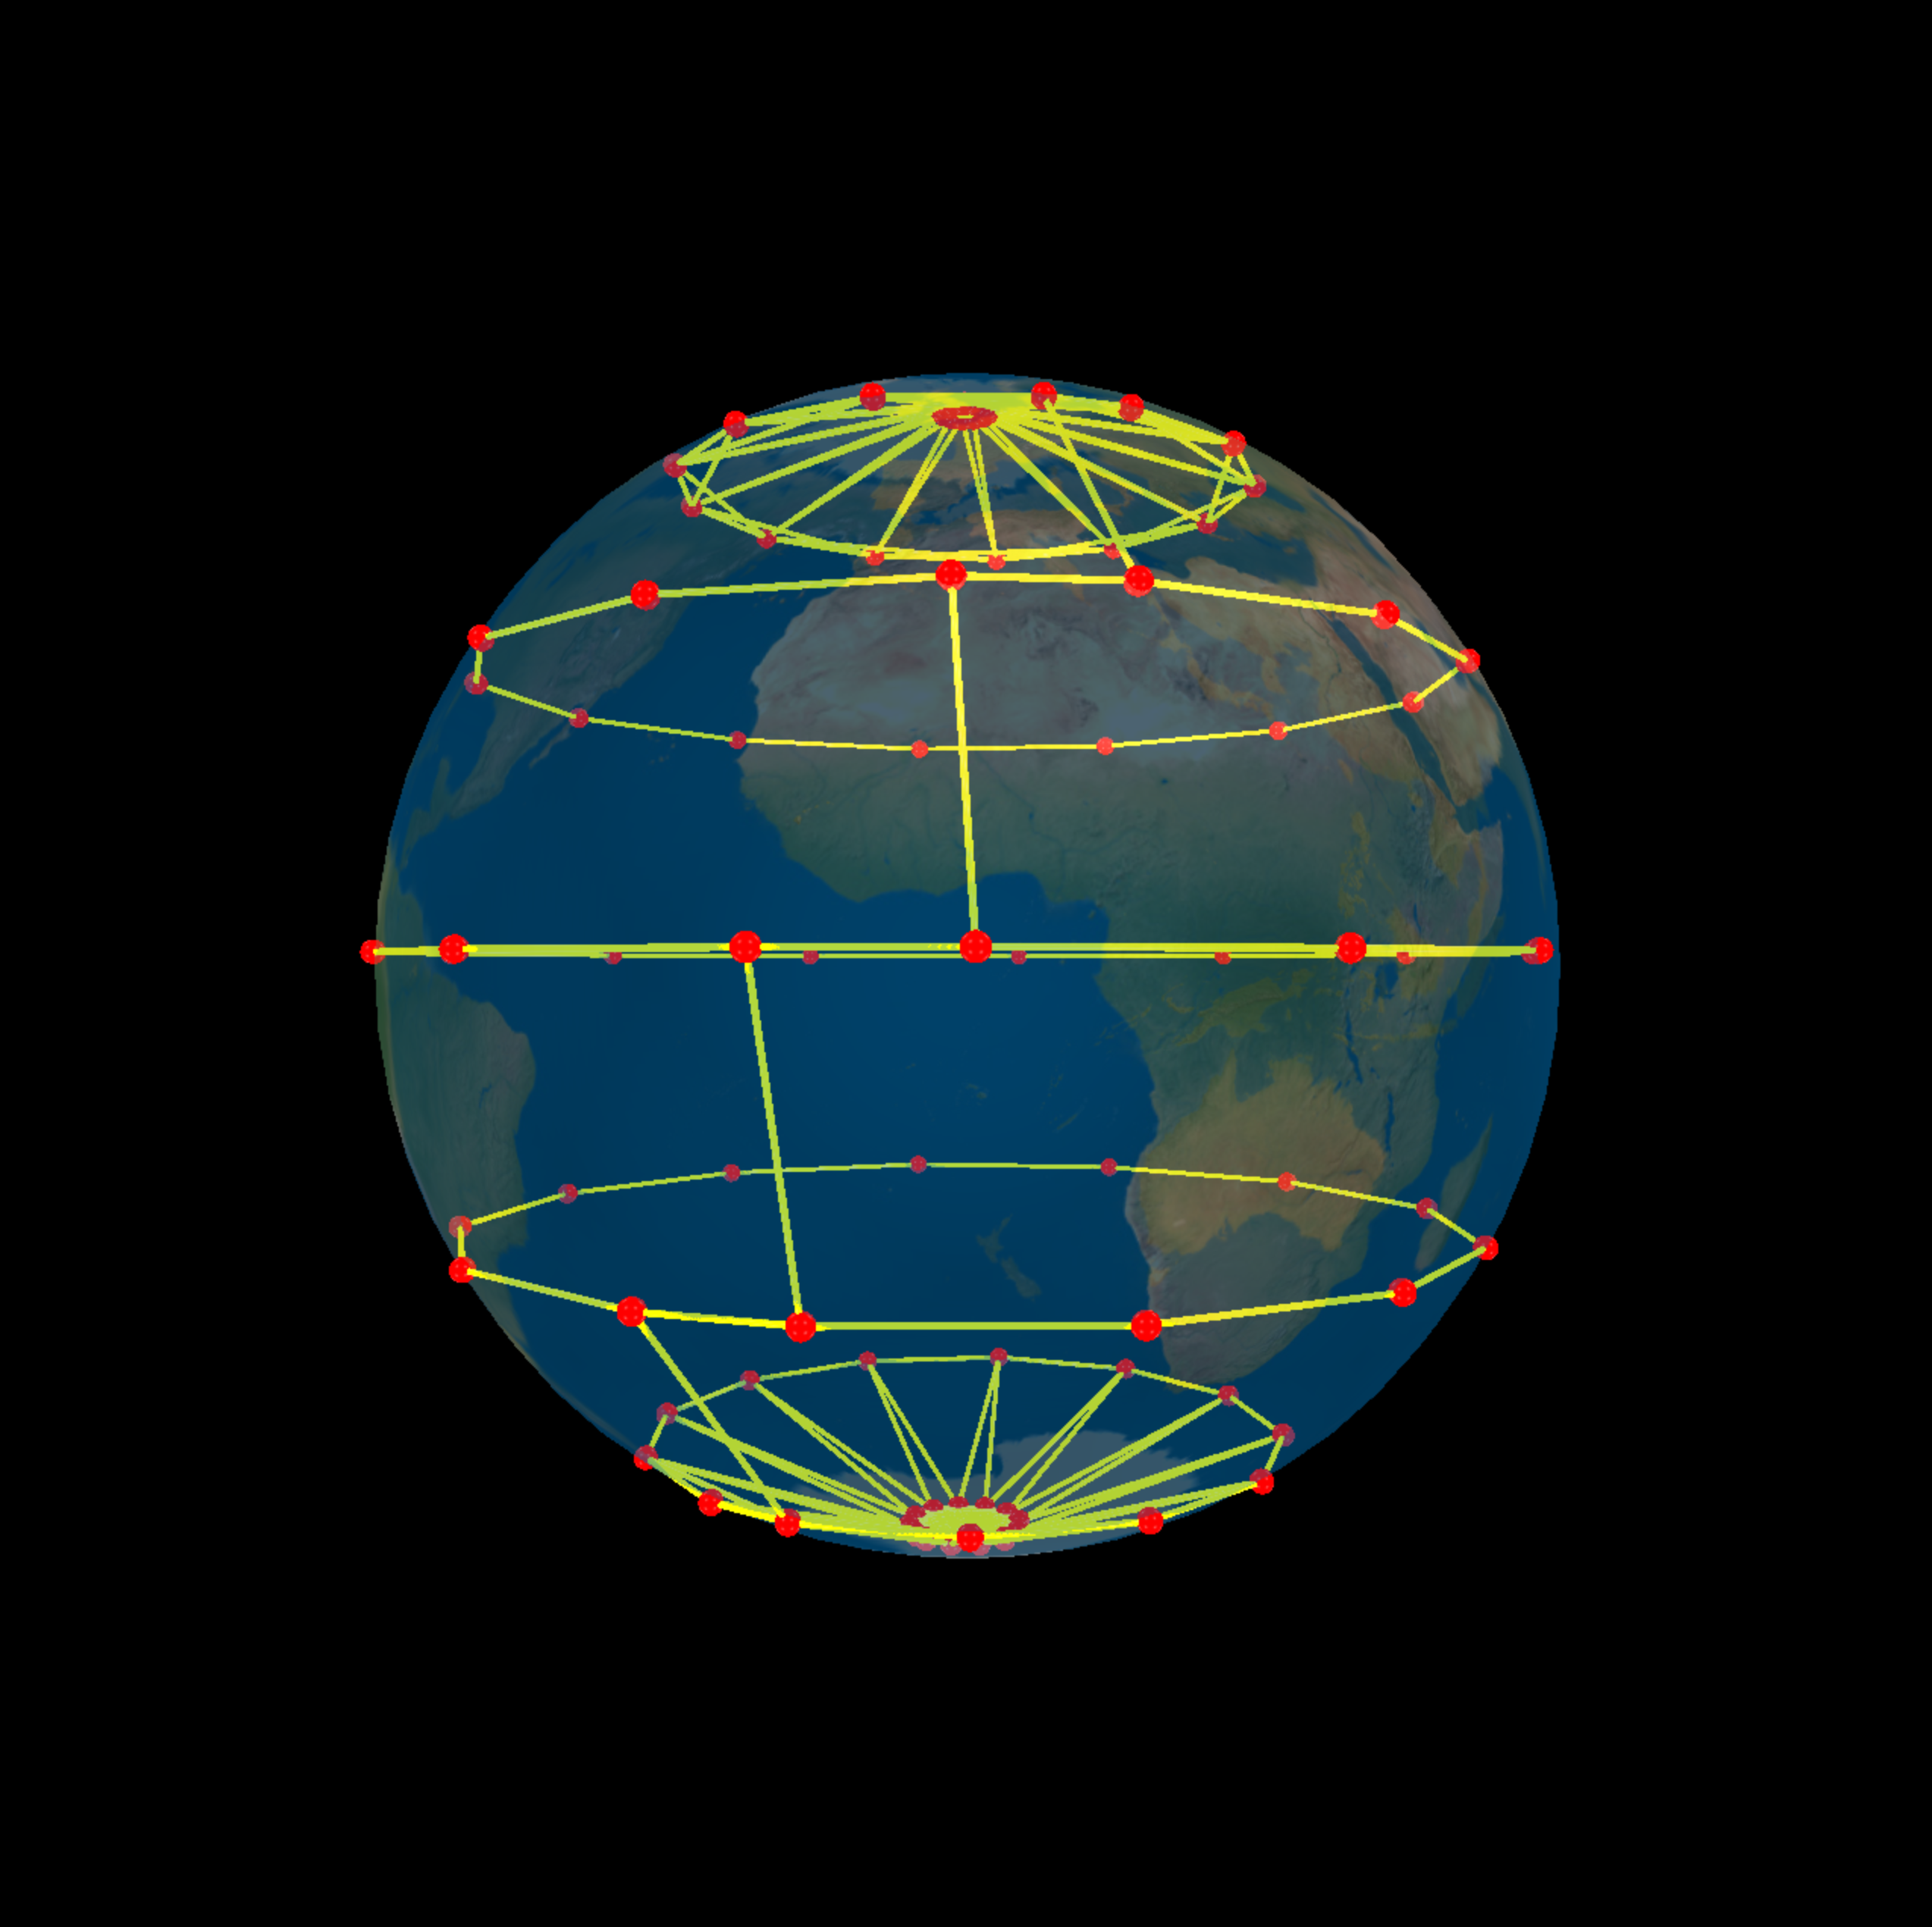
\includegraphics[width=\textwidth]{../images/connections02}
                \caption{sensors02.txt ($r=0.5$)}
            \end{subfigure}
        }
        \caption{Connections between sensors}
        \label{connections}
\end{figure}
In Figure \ref{connections} we can see the yellow edges of a Vietoris-Rips complex which connect sensors that can communicate. On the right picture we can also see the points around the poles, which we mentioned before, and have much shorter distances so they are also connected when $r$ is smaller.

\section{Coverage}
To determine the coverage of our sensor network we computed multiple Čech complexes with multiple $R$ parameters and looked at their first two Betti numbers. 

\begin{figure}[H]
        \centering
        \makebox[\linewidth][c]{
        	\centering
            \begin{subfigure}[b]{0.5\textwidth}
                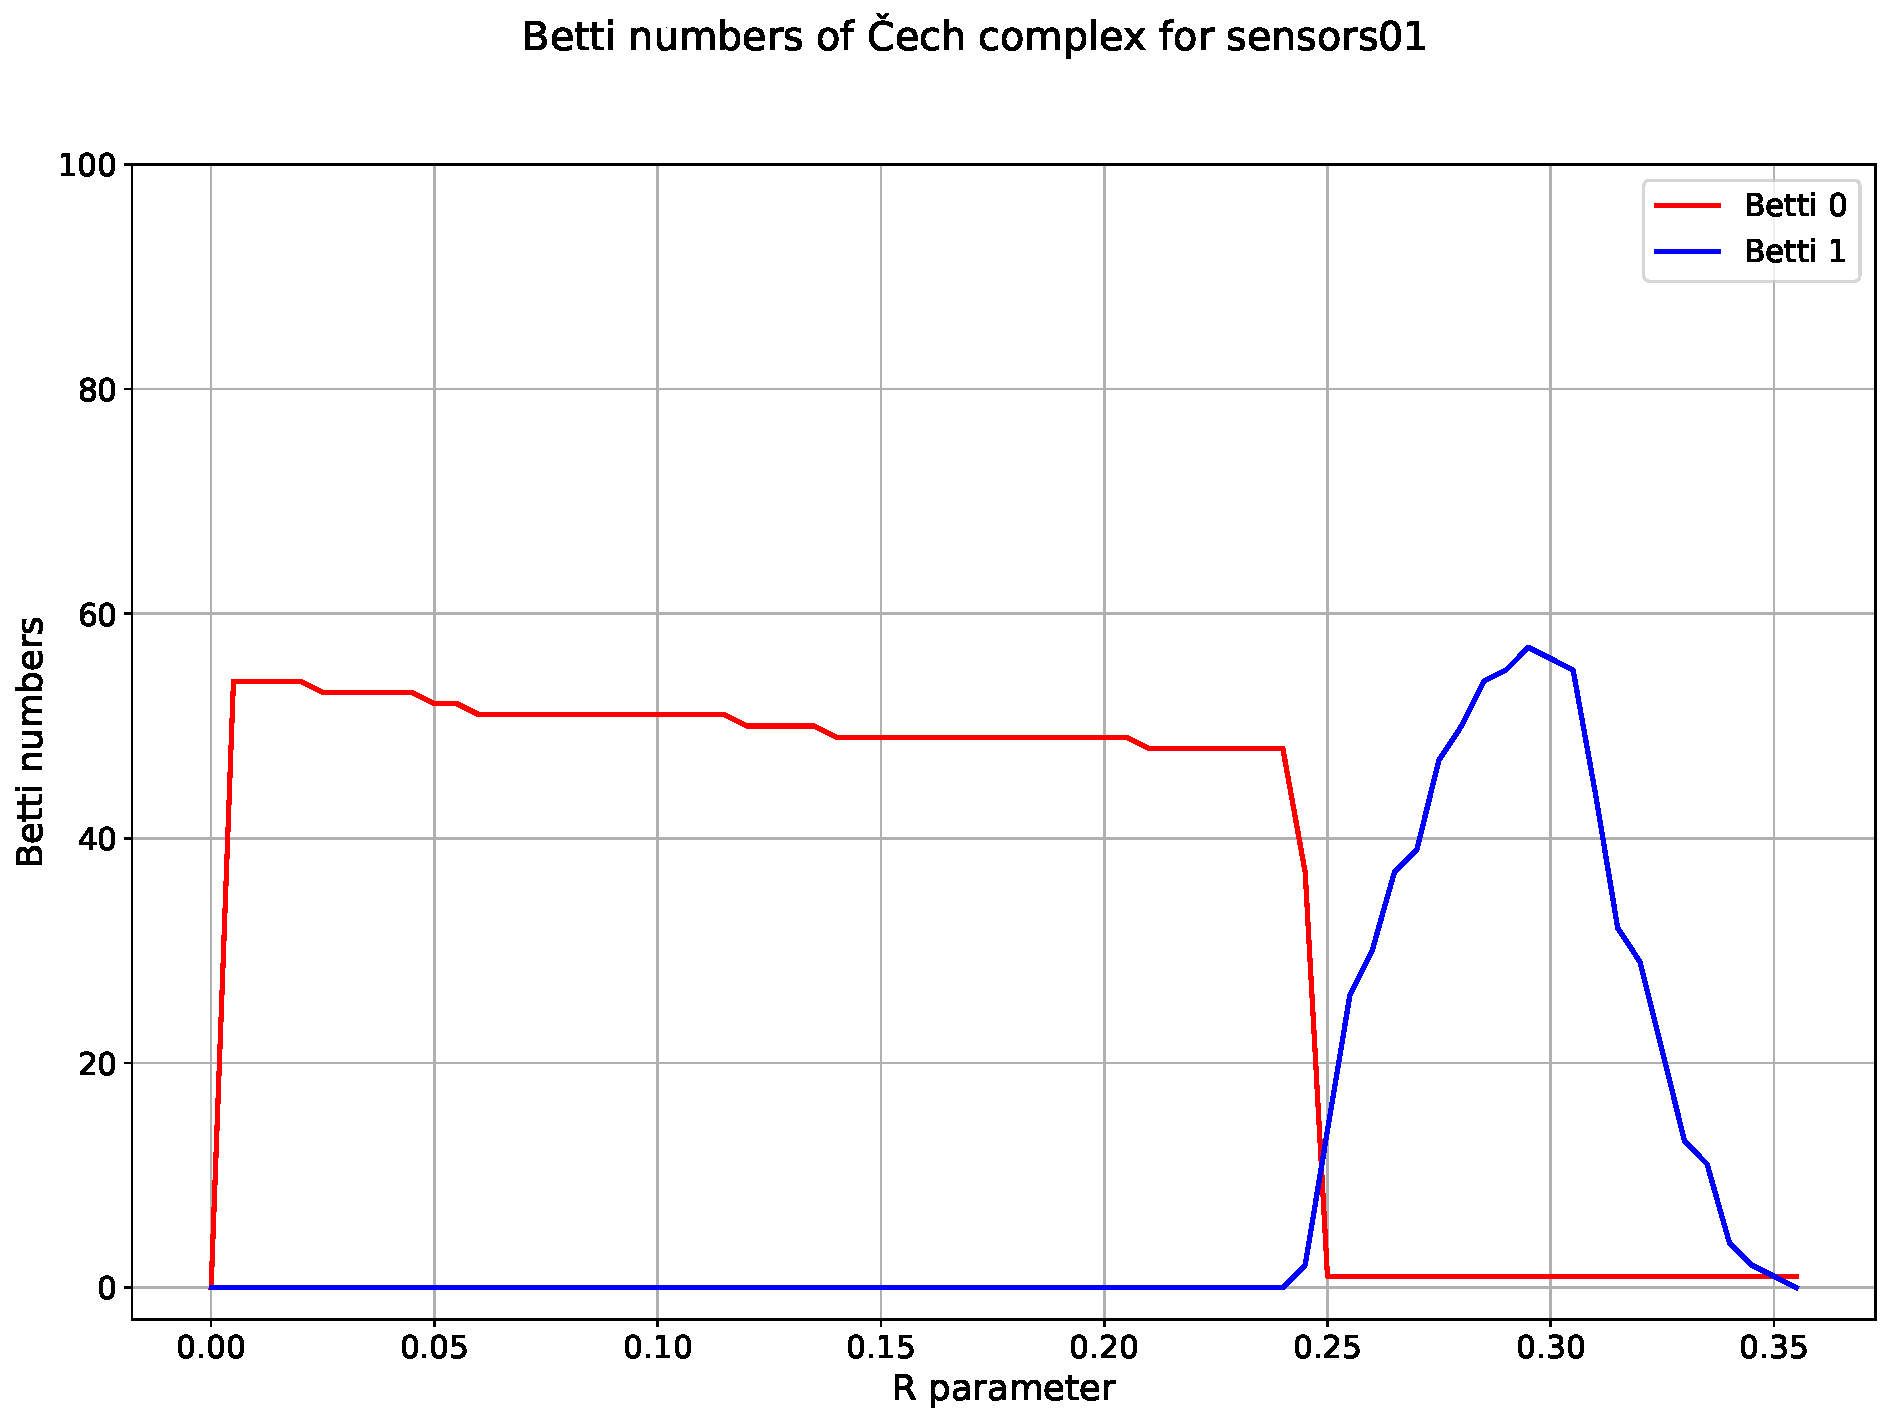
\includegraphics[width=\textwidth]{../images/plot_cech_sensors01}
            \end{subfigure}
            \begin{subfigure}[b]{0.5\textwidth}
                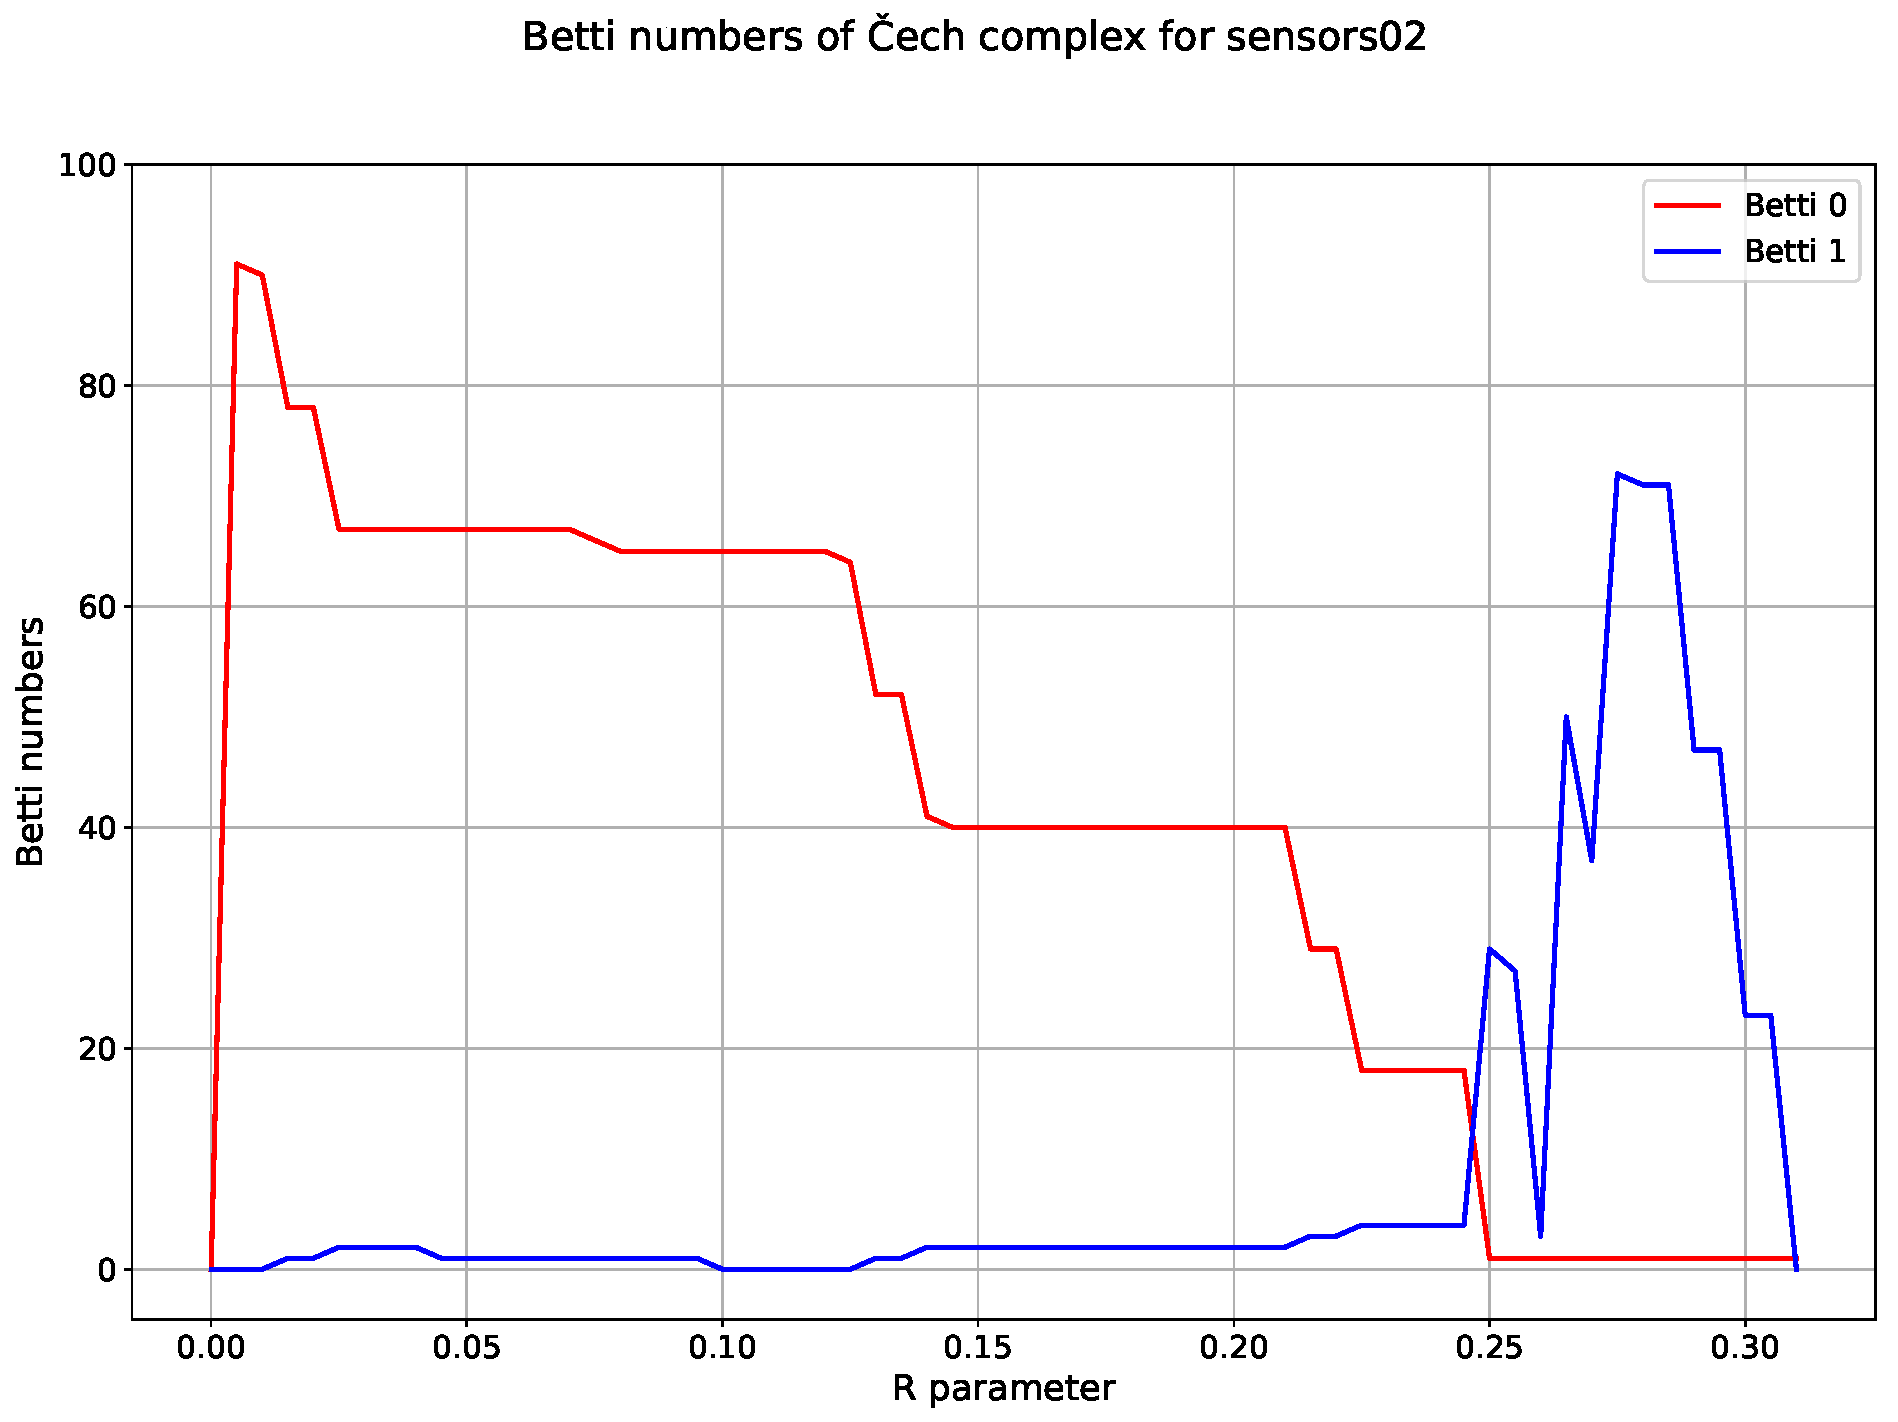
\includegraphics[width=\textwidth]{../images/plot_cech_sensors02}
            \end{subfigure}
        }
        \caption{$\beta_0$ and $\beta_1$ as we increase the $R$ parameter}
        \label{plot-cech}
\end{figure}
In Figure \ref{plot-cech} can see, that $\beta_0$, the number of components, represented by the red line has the same shape as on the previous Vietoris-Rips plots. We can also see that the blue line, the number of cycles in the complex, is low at first, rises when all the points are connected together and then decreases as the cycles turn into triangles. 

\begin{figure}[H]
        \centering
        \makebox[\linewidth][c]{
            \centering
        	\begin{subfigure}[b]{0.5\textwidth}
            	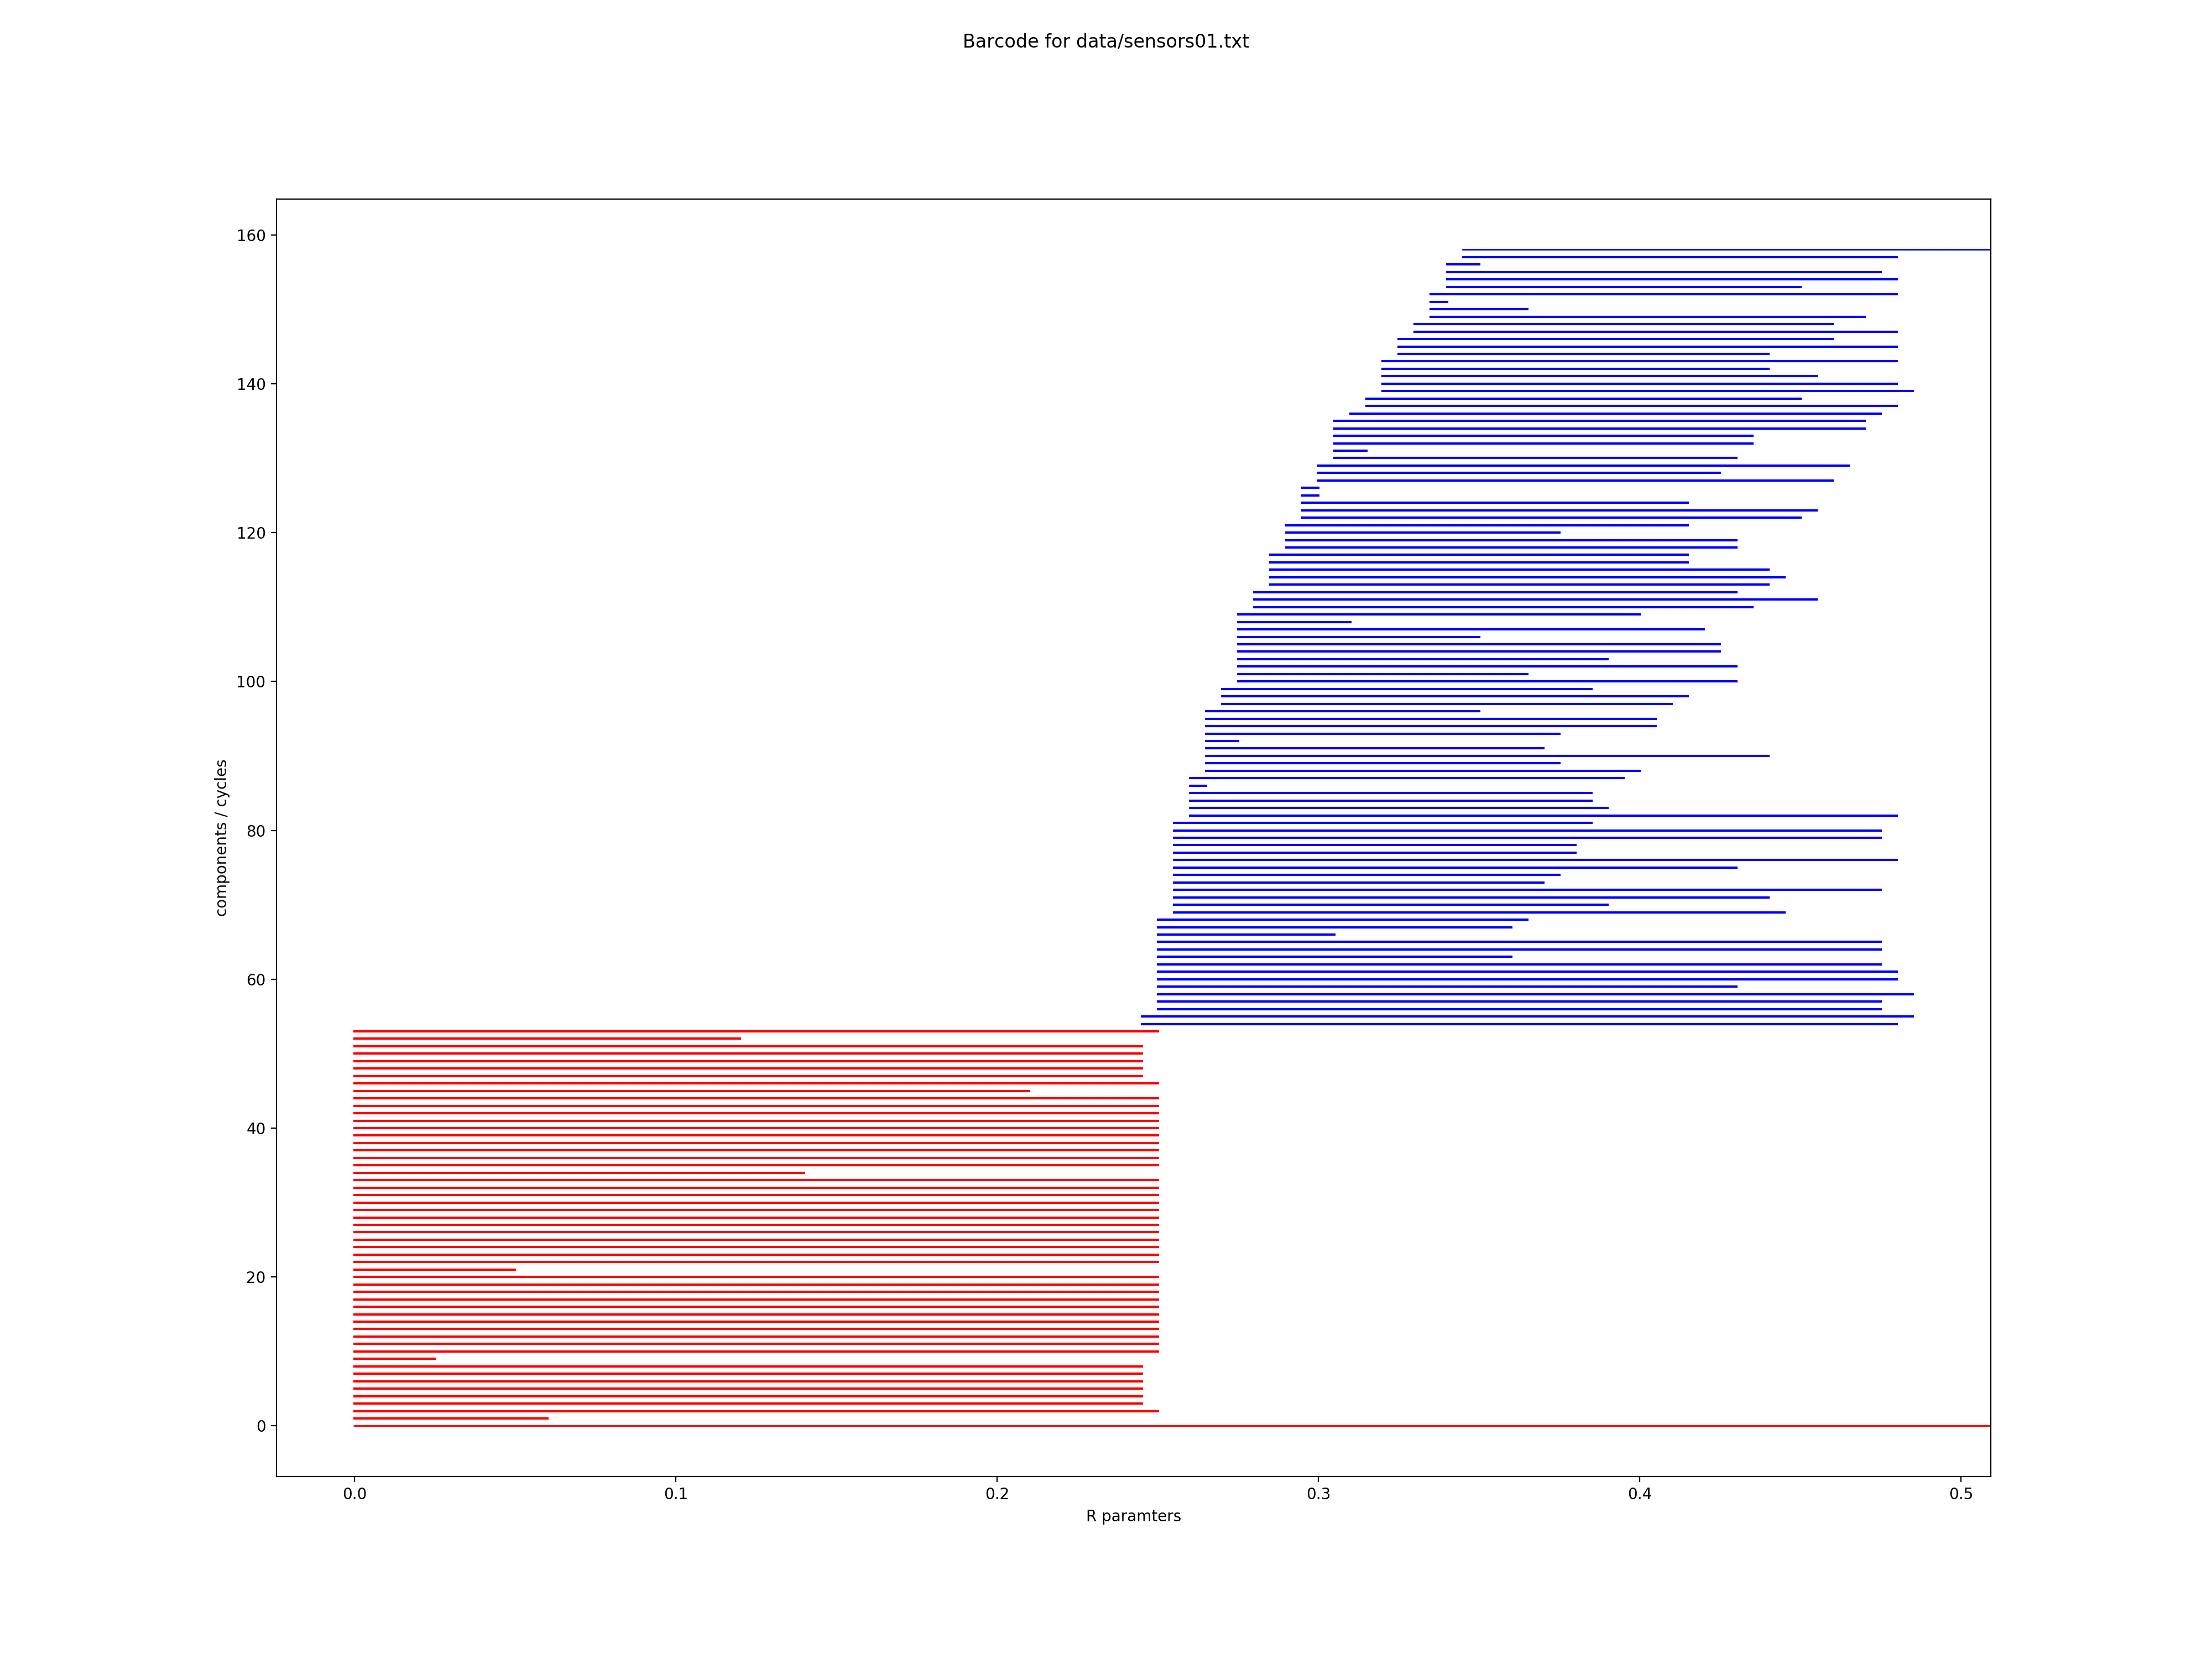
\includegraphics[width=\textwidth]{../images/barcode_cech_sensors01}
        	\end{subfigure}
			\begin{subfigure}[b]{0.5\textwidth}
            	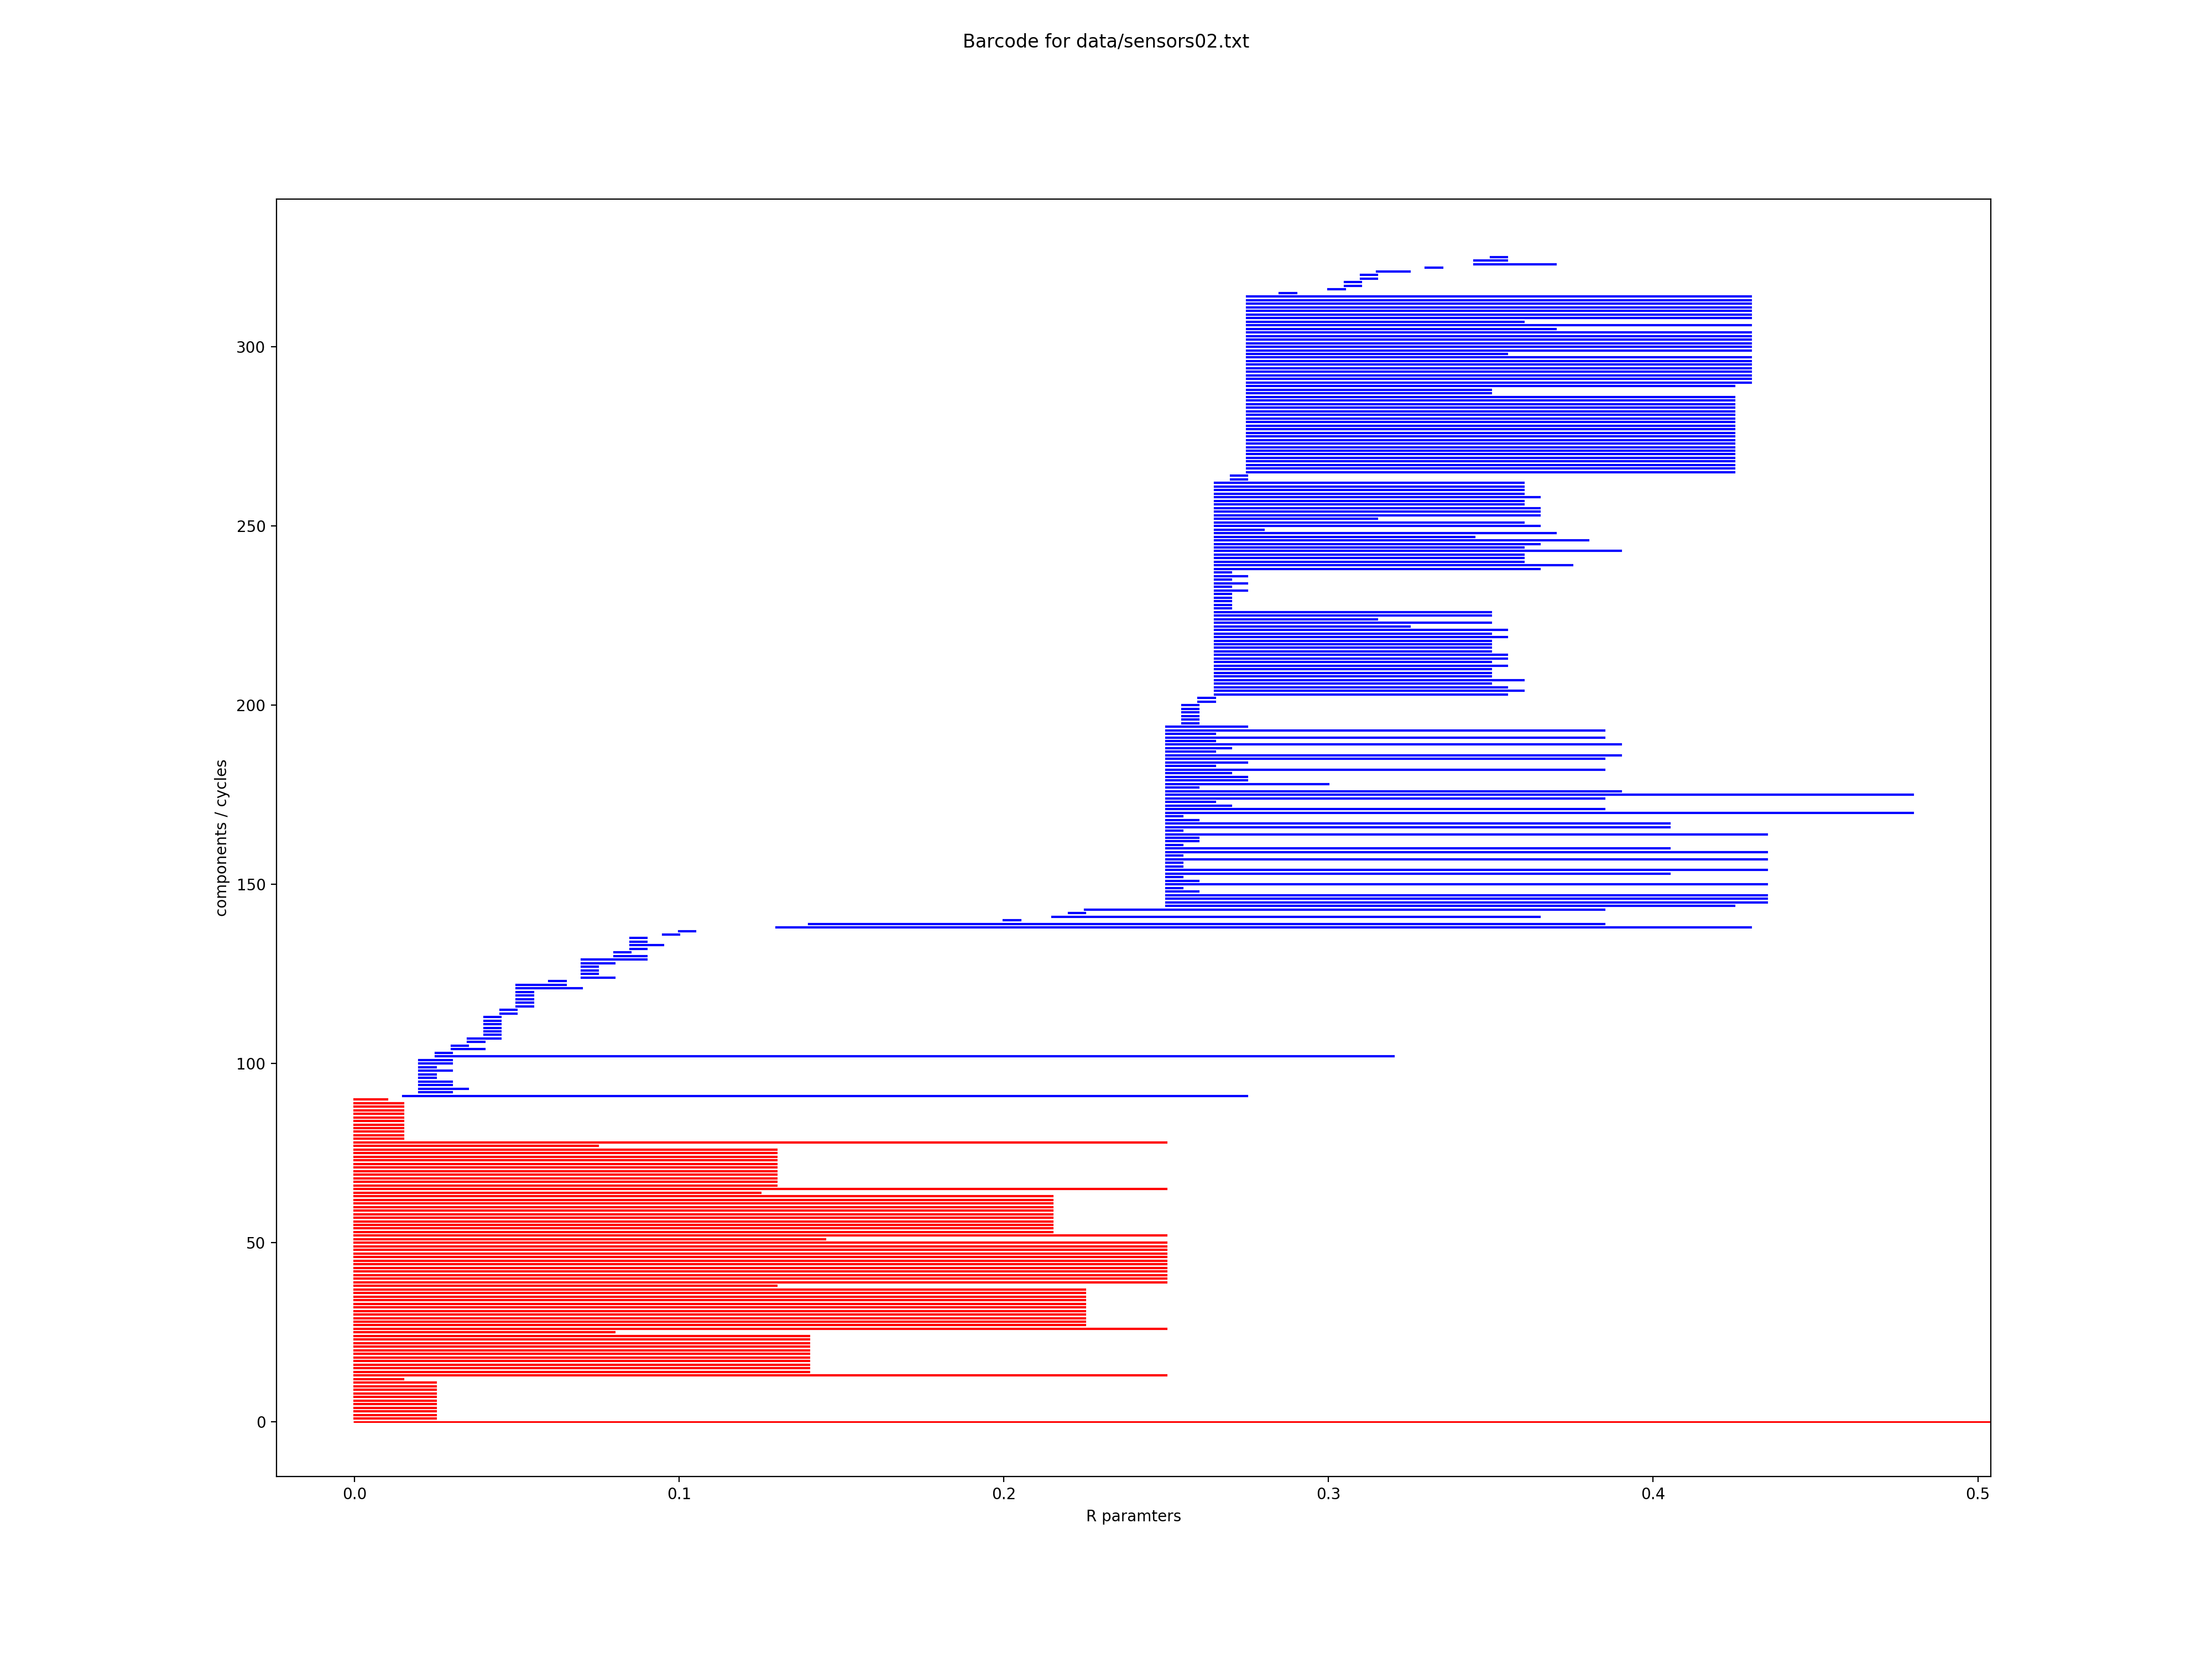
\includegraphics[width=\textwidth]{../images/barcode_cech_sensors02}
        	\end{subfigure}
        }
        \caption{Barcodes for the Čech complex}
        \label{barcodes}
\end{figure}
Barcodes in Figure \ref{barcodes} show us a very similar pattern.

\begin{figure}[H]
        \centering
        \makebox[\linewidth][c]{
        	\centering
            \begin{subfigure}[b]{0.55\textwidth}
        	    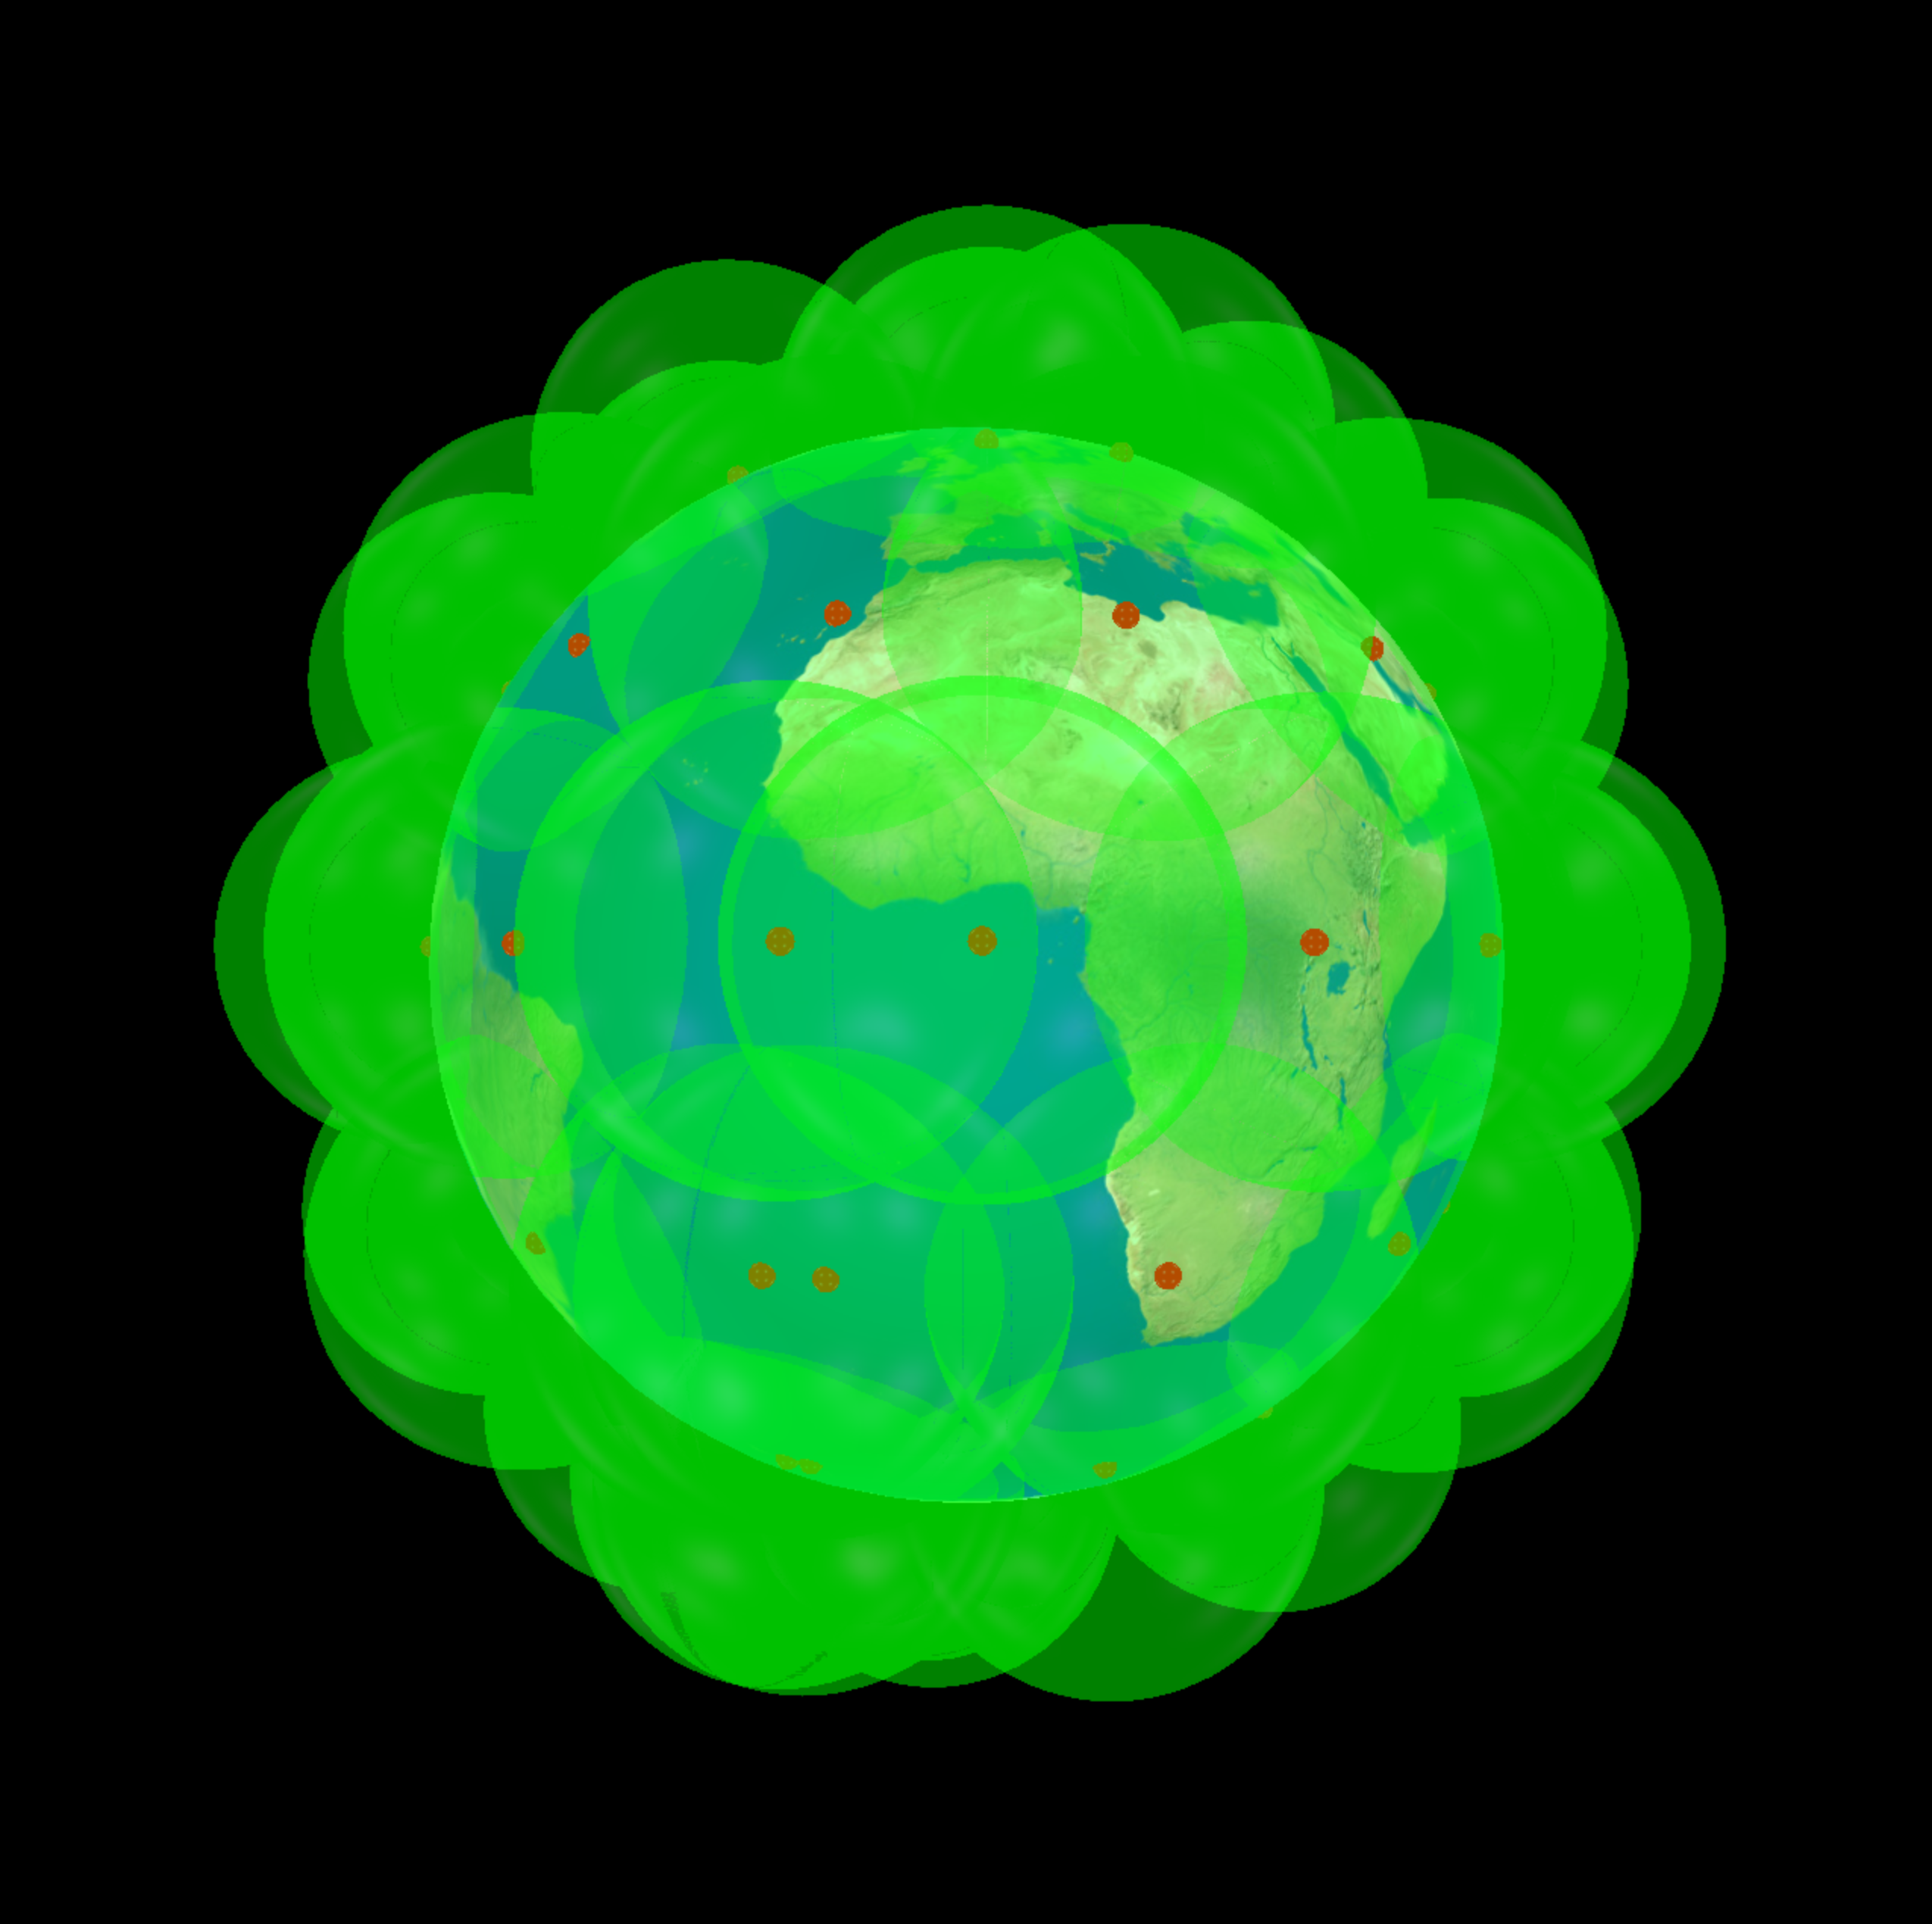
\includegraphics[width=\textwidth]{../images/coverage01}
        	    \caption{sensors01.txt ($R=0.355$)}
        	\end{subfigure}
        	\begin{subfigure}[b]{0.55\textwidth}
      	      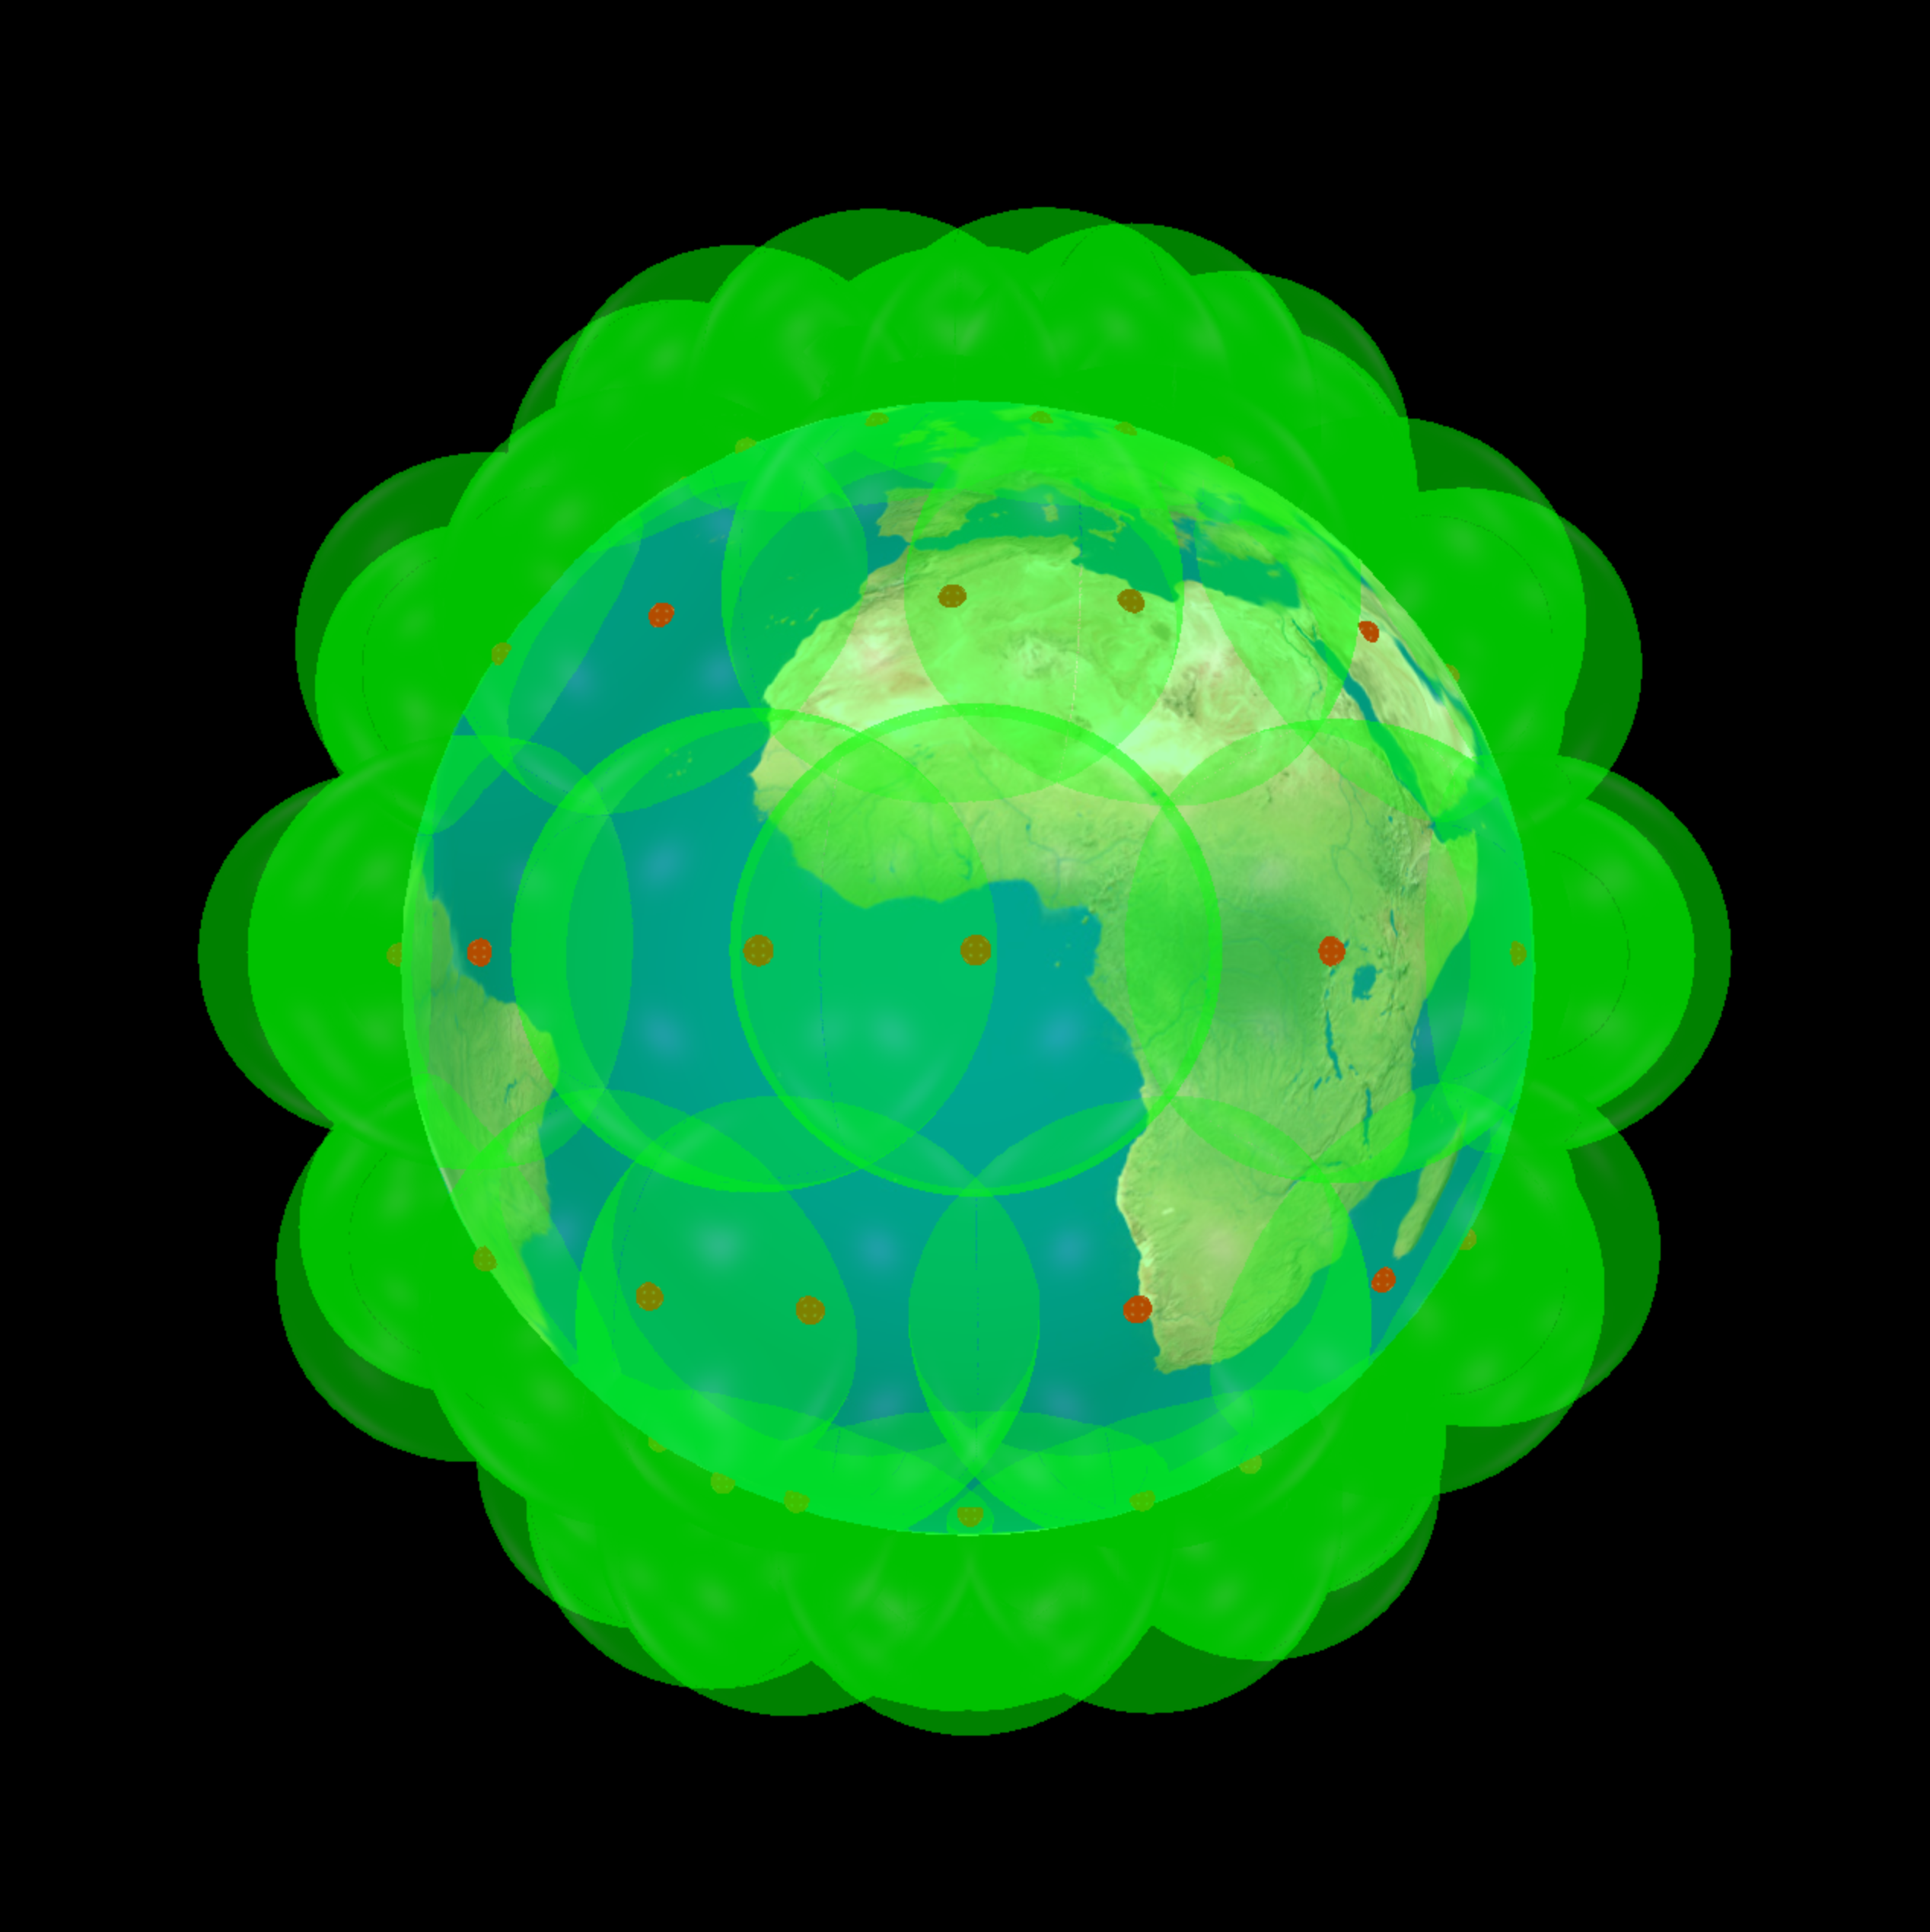
\includegraphics[width=\textwidth]{../images/coverage02}
     	       \caption{sensors02.txt ($R=0.31$)}
     	   \end{subfigure}
	  	}
        \caption{Connections between sensors}
        \label{coverage}
\end{figure}

In Figure \ref{coverage} we can see the coverage of each sensor, represented by a green ball with radius $R$ around it. We can see that there is some overlap between them (especially around the poles of the second dataset), but we can also see that decreasing the R would create holes in between some of the balls.


\section{Redundant sensors}
Once the parameters of the sensor network $r$ and $R$ were established, we had to find any redundant sensors. We first tried to go through all possible combinations ($n!$), which turned out to be very time demanding, so we reduced the complexity with the following simple algorithm:
\begin{itemize}
	\item We ignored the cut vertices of the graph on the VR complex. Removing them would separate the network in multiple components.
	\item We ignored all sensors with less than 3 neighbors in radius $R$ around them. Removing them would create a hole in the Čech complex.
	\item We then randomly selected points from the remaining list and removed them from the network if it was safe to do so (we checked if the remaining network would still satisfy the requirements).
\end{itemize}

The best solution that we got by randomly picking points from the complex was further improved by going through all the possible combinations of remaining sensors that could be safely removed. This was now faster, since we already removed most of the vertices that could be removed in the previous step. In the end, our algorithm for optimizing the sensor network was a compromise between finding a good solution and time needed for computation.


\section{Data generator}
Lastly, let us have a look at the data generator that distributes $n$ points evenly on the surface of a sphere. In order to meet this requirement we should look at points as electrons that are bound on the surface (i.e they have a fixed radius in spherical coordinates). The natural state would be the state with the lowest electrostatic-potential energy $V$ (eq. (2)). This is due to the fact that electrons repel from each other according to Coulumbs inverse square law (eq. (1))

\begin{equation}
	|\vect{F_{ij}}| = k_e \frac{e^2}{|\vect{r_i}-\vect{r_j}|^2},
\end{equation}
\begin{equation}
	V = \sum_{i\neq j}V_{ij} \propto \sum_{i\neq j}\frac{1}{|\vect{r_i} - \vect{r_j}|},
\end{equation}
where $k_e$ is Coulumbs constant, $e$ charge of electron and $\vect{r_i}$ local vector for $i-th$ point. It should be emphasized that potential energy was determined as sum of inversed Euclidean distances between all points. 

\subsection{Simulated annealing}
In order to determine the minimum of electrostatic-potential energy (eq. (2)) we used algorithm for simulated annealing with some Monte-Carlo modifications. 

At the beginning we randomly distributed $n$ points on the surface of a sphere with radius $r$ and selected the initial temperature of the system $T$. In each iteration a random point was chosen (one point was fixed, so $n-1$ available) and moved according to Gaussian distribution with appropriate parameters ($\mu = 0$ and small enough $\sigma$). 

After that, the difference in energy $\Delta E$ was calculated. If the energy of newly distributed points was less than before (i.e. $\Delta E < 0$) the move was accepted. Otherwise ($\Delta E \geq 0$) the move was accepted with the probability $\exp(\frac{-\Delta E}{T})$. The higher the difference in energy the lower are chances that we accept the change. Similar for the temperature, the lower the temperature the lower is the probability for accepting a bad move. If for a certain temperature $T$ enough changes $N_T$ were accepted, we decrease the temperature $T$ for $\Delta T$.

\subsection{Generated datasets}

Figure \ref{generated} shows two generated datasets, for $n = 4$ and for $n = 50$. We can see that in case of four points they distribute themselves in vertices of a tetrahedron and for $n = 50$ we get nice homogeneous even distribution of points.

\begin{figure}[!ht]
	\centering
	\begin{subfigure}{.5\textwidth}
		\centering
		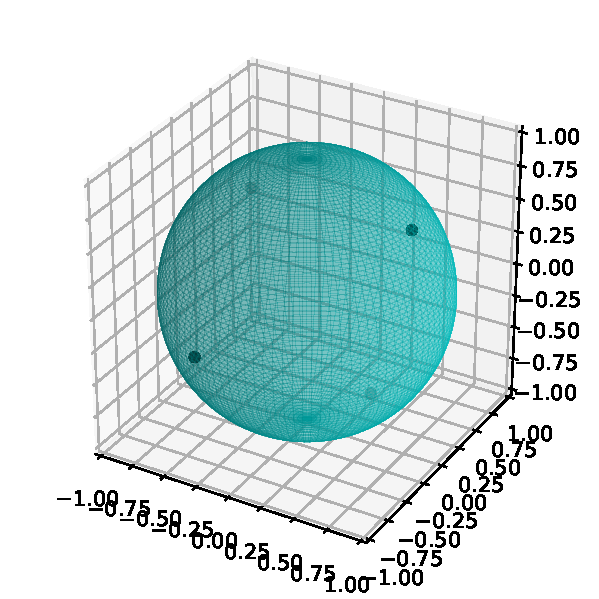
\includegraphics[scale=0.7]{../images/generated2.pdf}
		\caption{n = 4}
	\end{subfigure}%
	\begin{subfigure}{.5\textwidth}
		\centering
		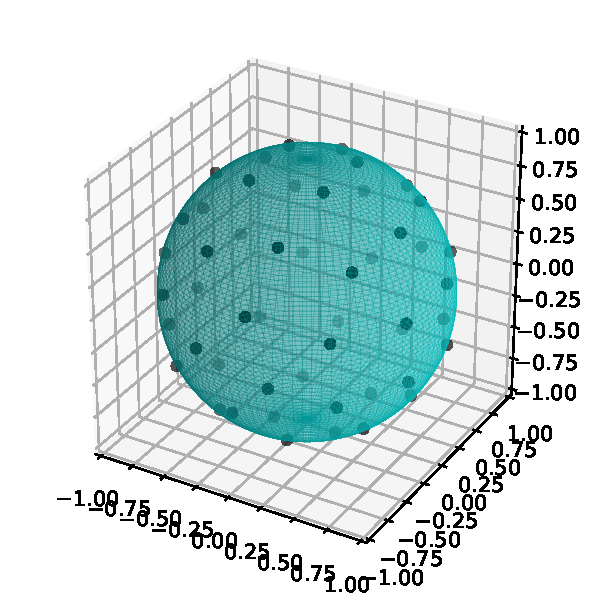
\includegraphics[scale=0.7]{../images/generated1.pdf}
		\caption{n = 50}
	\end{subfigure}%
    \caption{Even distribution of generated $n$ points on the surface of a sphere.}
	\label{generated}
\end{figure}


\section{Conclusion}

Topological data analysis is well suited for solving the problem of finding connections and coverage of a sensor network, since the definitions of connections in a graph and coverage of a sensor are essentially the same as definitions of edges in Vietoris-Rips and triangles in Čech complexes. The algorithms for computing the complexes are also fast enough that computing the solutions on the provided datasets takes just a few seconds.

An area that could be improved is the algorithm for finding redundant sensors, where we did not come up with any topological way of solving the problem. An idea that we thought about but did not explore in detail was to find simplices of a Čech complex with very high dimensions and reducing their dimension by removing sensors from them.


\clearpage

\begin{thebibliography}{99}
	\bibitem{} Vietoris-Rips. \url{https://en.wikipedia.org/wiki/Vietoris_Rips_complex} (5.6.2018).
	\bibitem{} Čech-complex. \url{https://en.wikipedia.org/wiki/Cech_complex} (5.6.2018).
	\bibitem{} Dionysus. \url{http://www.mrzv.org/software/dionysus/} (5.6.2018).
	\bibitem{} Miniball algorithm. \url{https://github.com/weddige/miniball} (5.6.2018).
	\bibitem{} Vpython. \url{http://vpython.org/} (5.6.2018).
	\bibitem{} Lecture notes from prof. dr. Neža Mramor Kosta and notes from the lab work.
\end{thebibliography}


\end{document}
